\PassOptionsToPackage{dvipsnames,usenames}{xcolor}


\documentclass[titlepage]{article} 

\usepackage{./style/ferinPackages}

% TITLE %%%%%%%%%%%%%%%%%%%%%%%%%%%%%%%%%%%%%%%%%%%%%%%%%%%%%%%%%%
\title{
%\normalfont \normalsize 
\large APPM 2360 Spring 2022 \\
[10pt] 
\rule{\linewidth}{2pt}  \\[10pt]
\huge Project 1 \\
\LARGE A Mathematical Investigation of the Heating and Cooling of Buildings\\
\rule{\linewidth}{2pt}  \\[10pt]
\author{Ferin Von Reich, Ben Scheck, Aaron Groudan}
\date{February 22, 2022}
}

%COMMANDS BEFORE BEGIN %%%%%%%%%%%%%%%%%%%%%%%%%%%%%%%%%%%%%%%%%%%%%%%%%
\doublespacing

%BEGIN DOCUMENT %%%%%%%%%%%%%%%%%%%%%%%%%%%%%%%%%%%%%%%%%%%%%%%%%%%%%%%%%%%%%%%%%%%%%%%%
\begin{document}
\definecolor {processblue}{cmyk}{0.96,0,0,0}
\maketitle

%TABLE OF CONTENTS %%%%%%%%%%%%%%%%%%%%%%%%%%%%%%%%%%%%%%%%%%%%%%%%%%%%%%%%%%%%%%%%%%%%%%%%%%%%%%%%
\tableofcontents
\newpage
%%%%%%%%%%%%%%%%%%%%%%%%%%%%%%%%%%%%%%%%%%%%%%%%%%%%%%%%%%%%%%%%%%%%%%%%%%%%%%

\section{Introduction}
When constructing a building, one must consider the heating properties. To do this, 
it is useful to consider the building as a singular compartment, and model the heat within the building. 
We will say that $T(t)$ in $\degree F$ represents the heat in the building at time $t$ in hours. 
Then, we can model the rate of change of the temperature inside the building $\frac{dT}{dt}$ in $(\degree F/hr)$, 
using the three main factors that generate or dissipate heat. Thus,
\begin{equation}\label{T_basic}
\frac{dT}{dt} = A(t) + H(t) + Q(t) 
\end{equation}
where $A(t)$ is the effect of the ambient outside temperature, $H(t)$ is the heat produced by people, machinery, 
and lights within the building, and $Q(t)$ is the effect of artifical heating and cooling from
furnaces and air conditioners.

In this project we will assign certain forms to $A(t), H(t)$ and $Q(t)$  and then explore
the implications of those forms, both separately as well as in the context of the model 
given by Eq. \eqref{T_basic}


%%%%%%%%%%%%%%%%%%%%%%%%%%%%%%%%%%%%%%%%%%%%%%%%%%%%%%%%%%%%%%%%%%%%%%%%%%%%%%
\section{Defining a Functional Form for A(T)}
To determine the functional form of $A(t)$ we will model the effects of the temperature of the air surrounding the 
building using Newton's Law of Cooling. This law states that the rate of change of the temperature of an object 
is directly proportional to the difference between the object's temperature, T(t), 
and the temperature of surroundings of the object. For this lab we will denote this using $M(t)$ which represents 
the ambient outside temperature. This means
\begin{equation}\label{A(t)}
    A(t) = \kappa[M(T)-T(t)]
\end{equation}
where $\kappa$ (the Greek letter kappa) is a positive constant of proportionality, indpendent of $M(t), T(t)$, and $t$, which determines how much the 
difference between the ambient temperature and the inside temperature affects $\frac{dT}{dt}$

%%%%%%%%%%%%%%%%%%%%%%%%%%%%%%%%%%%%%%%%%%%%%%%%%%%%%%%%%%%%%%%%%%%%%%%%%%%%%%
\section{Analysis of the Basic Form of T(t)}

\subsection{Finding and Analyzing the Basic Form of T(t)}\label{Linear T(t)}
When we substitute Eq.\eqref{A(t)} into Eq. \eqref{T_basic}, we find the following general differential 
equation modeling the rate of change of temperature within the building:
\begin{equation}\label{T_general}
    \frac{dT}{dt} = \kappa[M(T)-T(t)] + H(t) + Q(t) 
\end{equation}
Looking at this differential equation, assuming that $M(t), Q(t)$ and $H(t)$ are functions of $t$ only, 
we can make some observations. The equation is clearly linear, nonhomgeneous, and has constant coefficents. 
In addition, if $M'(t), Q'(t)$ and $H'(t)$ are continuous for all $t$, then by Picard's Existence and Uniqueness
Theorem there exists a unique solution to the differential equation for 
any initial condition. As an interpretation, if the solution given any initial condition exists and is unique, that simply
means that the temperature is determinsitc and predictable, implying that we can model the temperature using our equation.

Analyzing Eq. \eqref{T_general} given the special case where $Q(t) = tT$ (which we will later see is closer to the 
real model, Section \ref{furnaces and aircon}), we see only two differences from above. For one, the differential equation
would now have varible coefficents. Secondly, we would need to additionaly show that $Q_T(t)$, the partial derivative of $Q(t)$ 
with respect to $T$ was continous for all $T$ and $t$ to show that there exists a unique solution for the differential equation for 
any initial condition.


For further analysis, if we assume that  $M(t), H(t)$ and $Q(t)$ are functions of $t$ only
and are integrable for all $t$ then we can find the general solution of Eq. \eqref{T_general}
which may clue us into its behavior. To do this, we use use the integrating factor method on
Eq. \eqref{T_general} (see Appendix \ref{calc:integrating factors} for calculation) which produces
\begin{equation}\label{eq:integrating factor}
    T(t) = e^{-\kappa t}\int _{t_0}^t\:[\kappa M(s)+H(s)+Q(s)]e^{\kappa s}ds +e^{\kappa (t_0-t)} T_0        
\end{equation}

\subsection{Inspecting a Simplified T(t)}
To analyze the basic behavior of $T(t)$, let us first consider a case in which the building 
has no people in it, lights and machinery are off, no furnaces or air conditoners are running, 
and the outside temperature is constant. In other words, $H(t) = 0, Q(t) = 0, \text{ and } M(t) = M_0$.
Applying these assumptions to Eq. \eqref{T_general}, we get the following:
\begin{equation} 
    \frac{dT}{dt} = \kappa[M_0-T(t)]
\end{equation}
From this equation we can determine if there are any equilibrium solutions, by setting $\frac{dT}{dt}=0$, which provide
a clue towards the long term behavior of the temperature inside the building.
\begin{align*}
    0 &= \kappa[M_0-T(t)]\\
    0 &= M_0-T(t) \\
    T(t) &= M_0 
\end{align*}
Thus, the equilibrium solution is $M_0$. In addition, if $T(t) > M_0, \text{ then } \frac{dT}{dt}<0$ and if
$T(t) < M_0, \text{ then } \frac{dT}{dt}>0$, meaning that $M_0$ is a stable equilibrium, so for any intial condition
the temperature inside the building for this situation will eventually settle at $M_0$.

To examine this situation further, we can apply the assumptions within it into Eq. \eqref{eq:integrating factor}, and the
initial condition $T(t_0)=T_0$  to solve the inital value problem for $T(t)$. This produces the following equation 
(see calculation in Appendix \ref{calc:analytical}):
\begin{equation}\label{eq:analytical}
    T(t) = M_0 + (T_0 - M_0 e^{\kappa (t_0-t)}) 
\end{equation}
This will allow us to test if our equilibrium solution makes sense. 
To do this we can graph Eq. \eqref{eq:analytical} with $M_0=75$, $t_0=0$, and $\kappa=0.25$ for both $T_0=50$ and $T_0=80$. 
Looking at Fig. \ref{fig:equilib1} we can see that our solution  for $T(t)$ confirms our stable equilibrium solution of $M_0=75$
since both curves converge to it.
\begin{figure}[H]
    \centering
    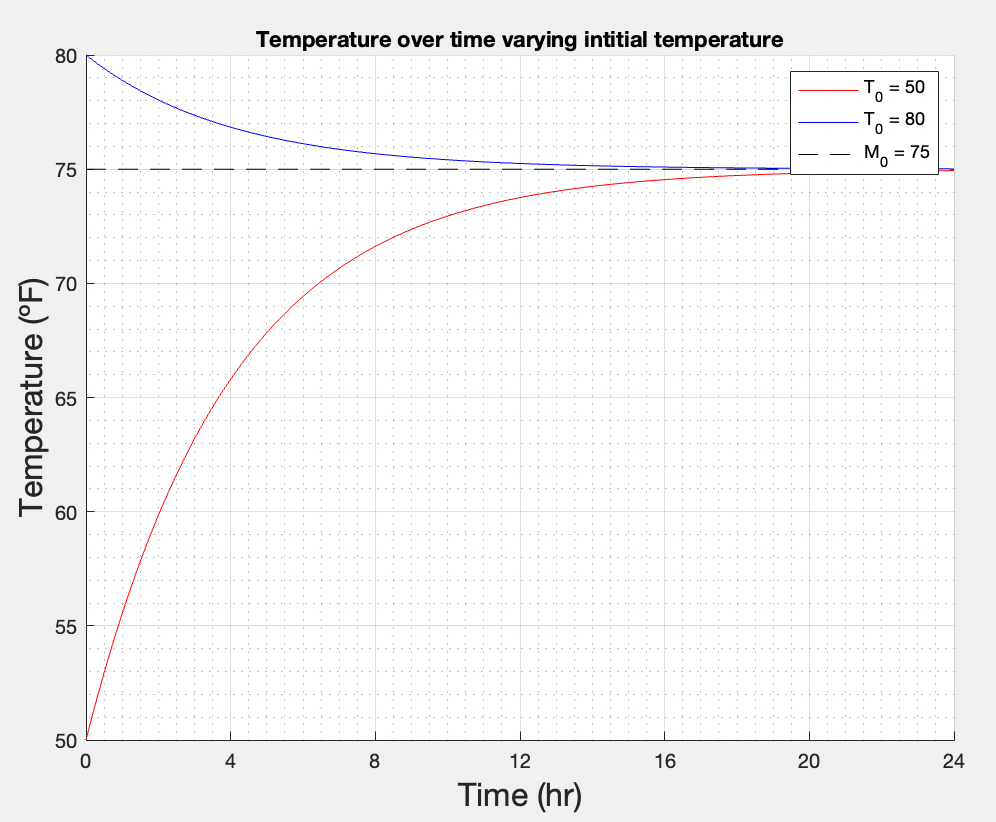
\includegraphics[width=0.6\textwidth]{./images/equilib1.png}
    \caption{Graph of Eq. \eqref{eq:analytical} with $M_0=75$, $t_0=0$, and $\kappa=0.25$ while varying $T_0$}
    \label{fig:equilib1}
\end{figure}

Having determined the equilibrium solution, it is also useful to consider how $\kappa$
affects $T(t)$ by graphing multiple solutions while varying $\kappa$. Looking at a graph of just
such a thing, Fig. \ref{fig:kappa} we can see that as $\kappa$ increases, the temperature converges 
to the equilibrium solution faster (meaning the rate of change increases). Thus, we could think of many physical ways to affect 
$\kappa$. For example, if we increased the number of windows then the building would be less insulated, so the temperature
would be more reactive to the outside temperature, meaning that $\kappa$ would be larger.
\begin{figure}[H]
    \centering
    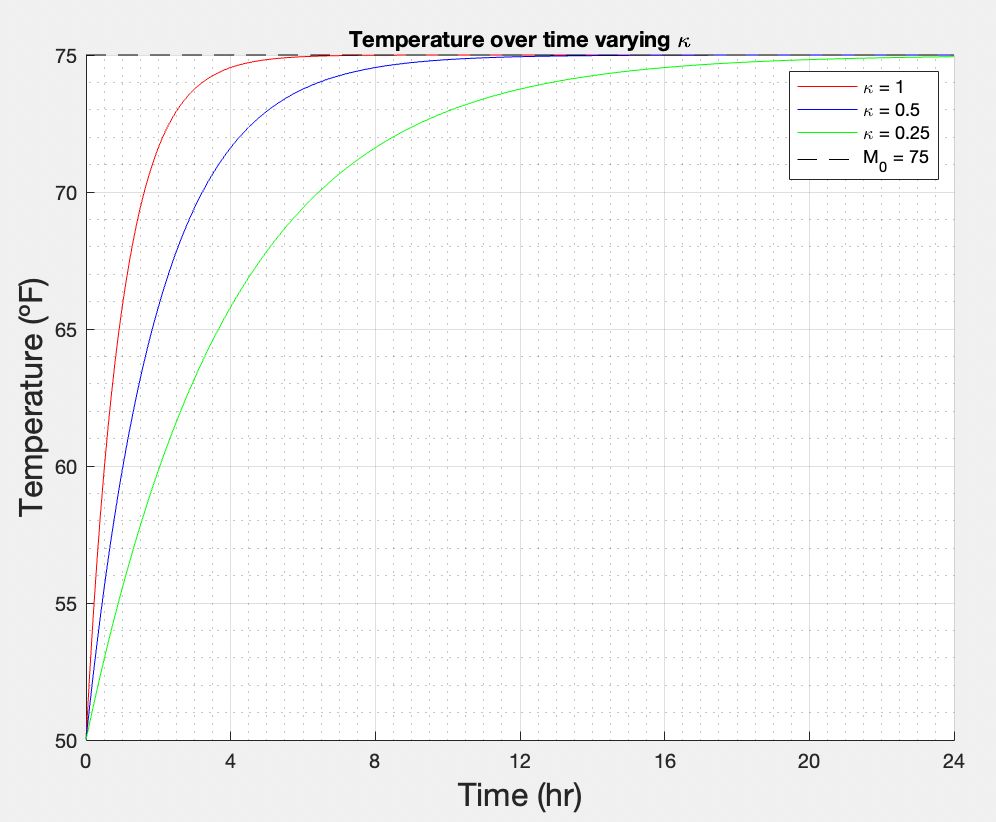
\includegraphics[width=0.6\textwidth]{./images/kappa.png}
    \caption{Graph of Eq. \eqref{eq:analytical} with $M_0=75$, $t_0=0$, and $T_0=0.50$ while varying $\kappa$}
    \label{fig:kappa}
\end{figure}

To complete our analysis of the basic form of $T(t)$, we can use the Eq. \eqref{eq:analytical} to find the value of the time constant, $\Delta t = t - t_0$, where $\Delta t$
is in hours, when the difference between the building's temperature and the outside temperature is $e^{-1}$ of the initial 
difference. To do this, we set $ e^{-1}(T_0-M_0) = T(t)-M(t)$, plug in an expression for $t$ and solve for $\Delta t$. See full calculation in
Appendix \ref{calc:time constant}. This gives us the time constant:
\begin{equation} \label{eq:time constant}
    \Delta t = \frac{1}{\kappa}
\end{equation}
Fom Eq. \eqref{eq:time constant}  we can see that that time constant is inversely related to $\kappa$. This leads to a potentially useful conclusion.
If one was designing a building and wanted internal temperature not to respond quickly, then one would
design the building with a small $\kappa$ (as was previously shown), which in turn would mean that
one would want $\Delta t$ to be proportionally large.


%%%%%%%%%%%%%%%%%%%%%%%%%%%%%%%%%%%%%%%%%%%%%%%%%%%%%%%%%%%%%%%%%%%%%%%%%%%%%%%%
\section{Approximation Using Runge-Kutta}
As we explore our model further, we will approximate solutions to differential equations
using numerical techniques. Thus, in this section we will quickly examine our programatic 
solution to solve first order inital value problems of the form $y'=f(t,y), y(t_0)=y_0 $ using the Runge-Kutta
Fourth Order Method. To view the MATLAB code directly see Appendix \ref{Runge-Kutta}.

To judge our solution, we will solve the initial value problem 
\begin{equation}\label{eq:runge}
    \frac{dT}{dt} = 0.25(75-T), T(0)=50
\end{equation}
on the interval $[0,24]$ (hrs) using $240$ points (stepsize $h = 0.1$), and compare our approximation to the real solution.
\begin{figure}[H]
    \centering
    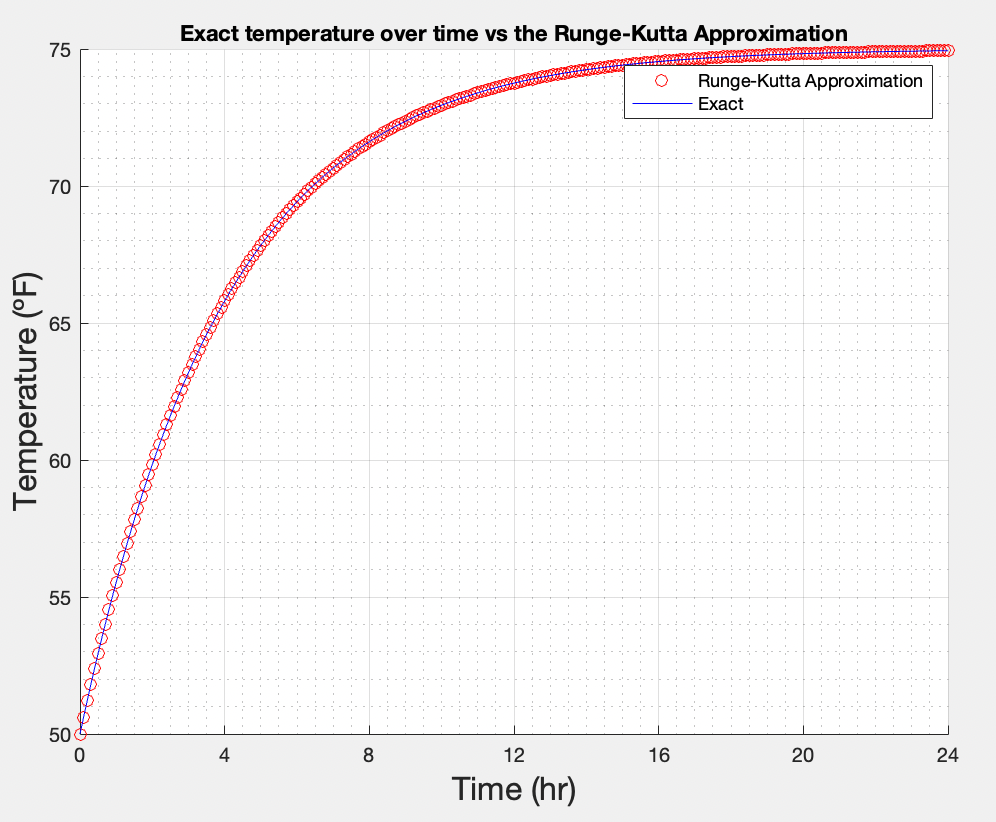
\includegraphics[width=0.6\textwidth]{./images/rungeKuttaExact.png}
    \caption{Graph of Runge-Kutta approximation and exact solution for Eq. \eqref{eq:runge}}
    \label{fig:rungeKuttaExact}
\end{figure}
As we can see from Fig. \ref{fig:rungeKuttaExact}, our approximate solution is almost identical to the exact solution.
In fact, looking at Fig. \ref{fig:rungeKuttaError} below, we can see that the error in our approximation is at worst around $(3*10^{-8})\degree F$. 
Thus, in the future when we solve such intial value problems, we will use this method.
\begin{figure}[H]
    \centering
    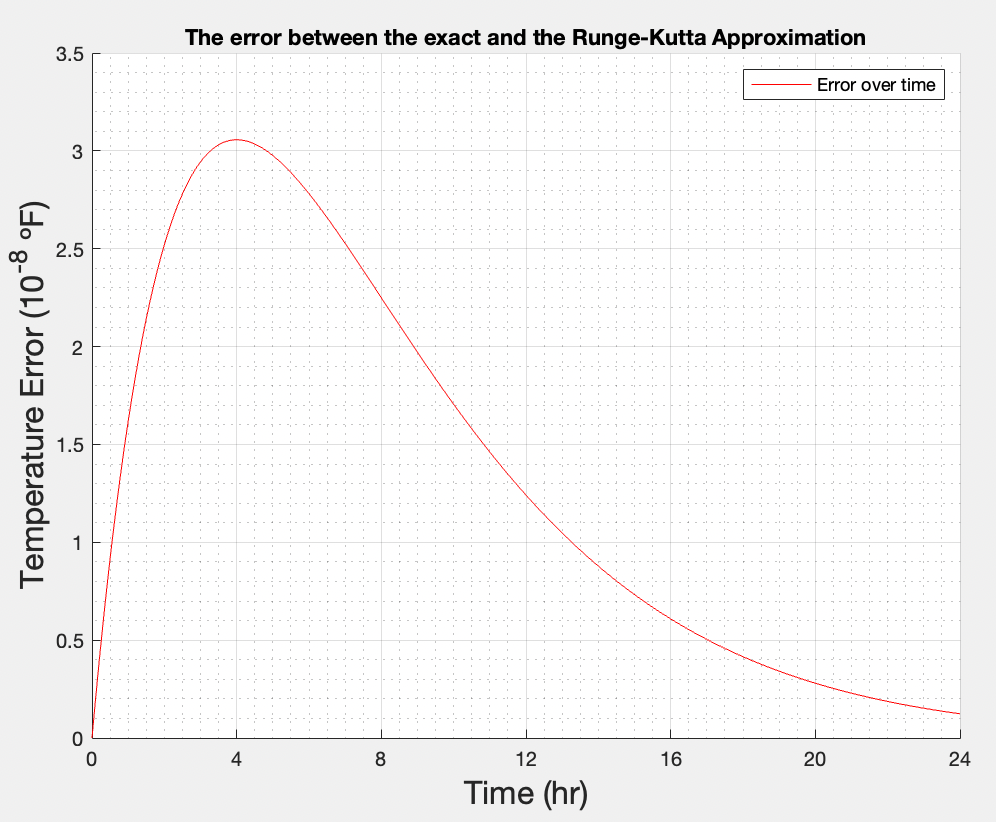
\includegraphics[width=0.6\textwidth]{./images/rungeKuttaError.png}
    \caption{Graph of the absolute difference between the Runge-Kutta approximation and exact solution for Eq. \eqref{eq:runge}, scaled by $10^{-8}$}
    \label{fig:rungeKuttaError}
\end{figure}



%%%%%%%%%%%%%%%%%%%%%%%%%%%%%%%%%%%%%%%%%%%%%%%%%%%%%%%%%%%%%%%%%%%%%%%%%%%%%%%%
\section{The Effect of the Outside Ambient Temperature}
Now we may consider the effect of the ambient temperature, $M(t)$, given a varying outside temperature
with no heating or cooling. In other words, let us assume that $H(t)=Q(t)=0$ and let us model $M(t)$ as follows:
\begin{equation}\label{eq:M(t)}
    M(t) = M_0 - 12\cos\left[\frac{\pi(t-5)}{12}\right]
\end{equation}
Substituting Eq. \ref{eq:M(t)} into Eq. \ref{T_general} subject to the assumptions above then leads to the following differential equation for this situtation.
\begin{equation} \label{eq:outsideTemp}
    \frac{dT}{dt} = \kappa[M_0 - 12\cos\left[\frac{\pi(t-5)}{12}\right]-T(t)] 
\end{equation}
Now, to analyze this situation, let us consider $T(t)$ and $M(t)$in two situations in which $T(0)=65$, and  $M_0=75 \text{ or } M_0 = 35$, so we can see how outdoor heat affects indoor heat.
\begin{figure}[H]
    \centering
    \subfloat[\centering $M_0=75\degree F$]{{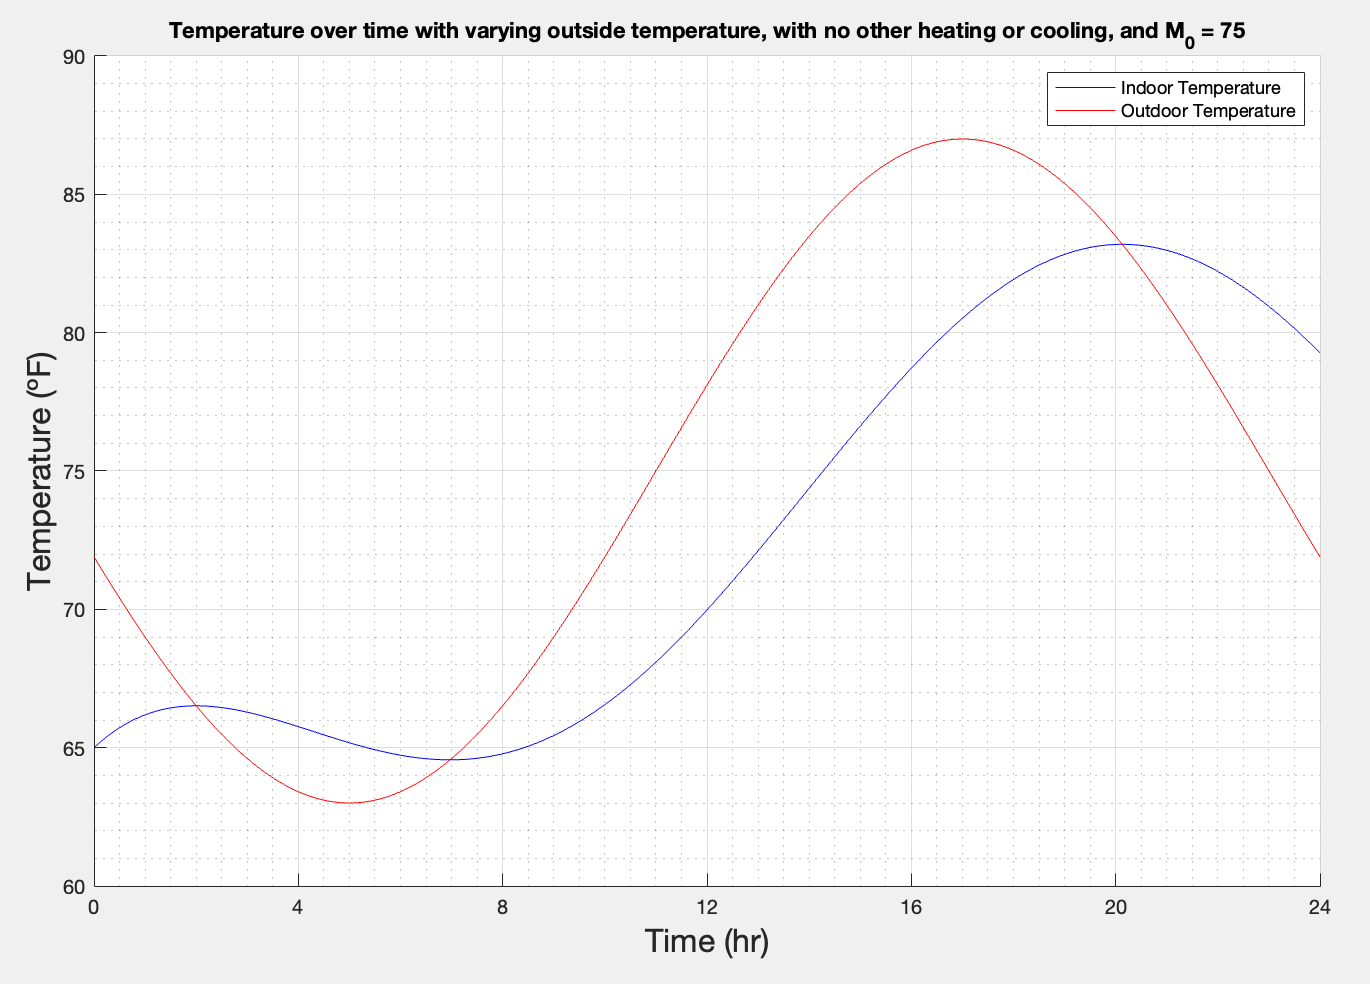
\includegraphics[width=0.4\textwidth]{./images/c75.png}}}%
    \qquad
    \subfloat[\centering $M_0=35\degree F$]{{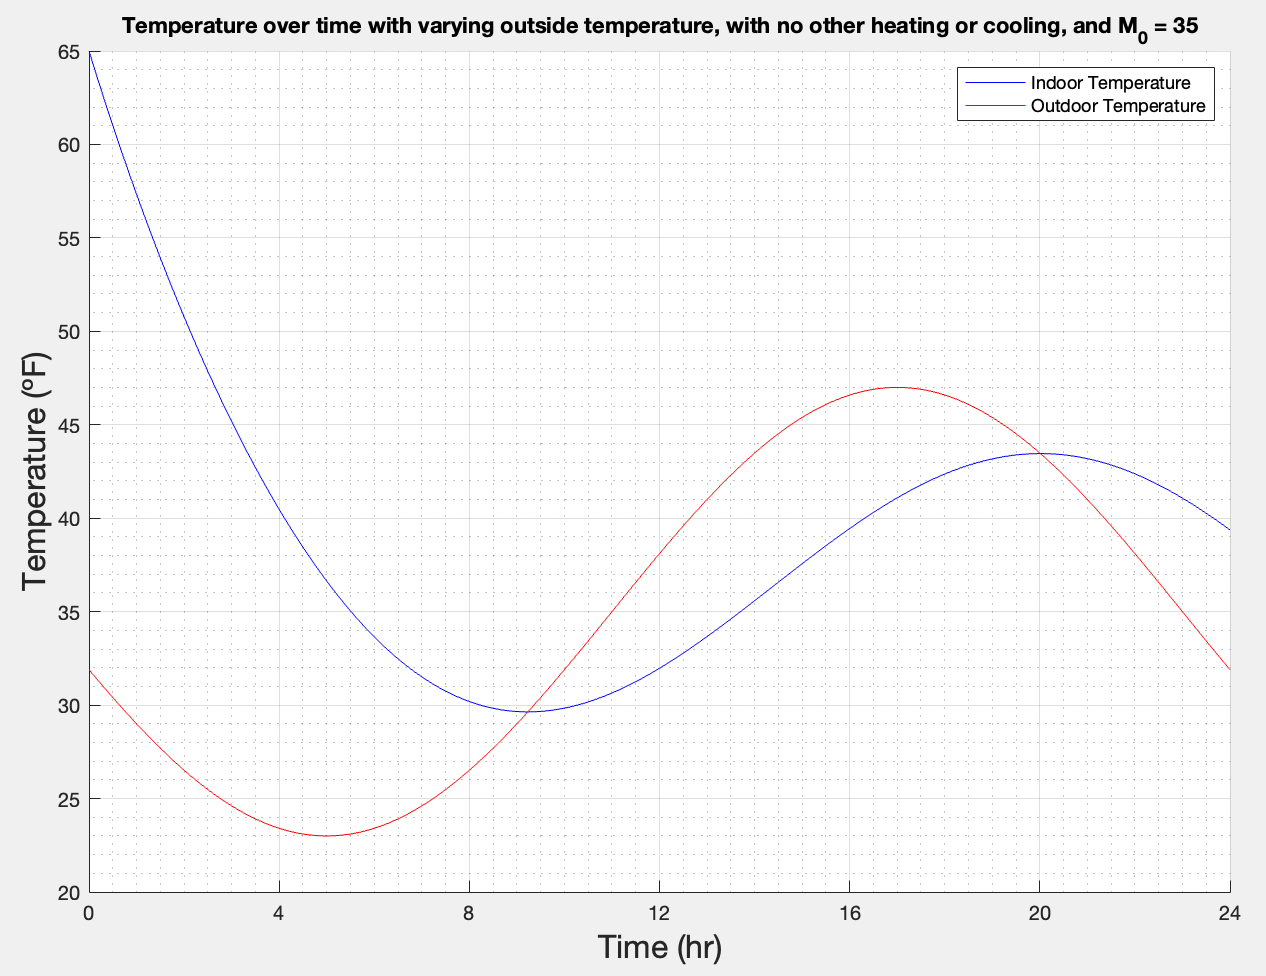
\includegraphics[width=0.4\textwidth]{./images/C35.png}}}%
    \caption{Solutions of Eq. \ref{eq:outsideTemp} plotted with $M(t)$ where $T(0)=65\degree F$}%
    \label{fig:outsideTemp}%
\end{figure}
Now that we have these plots, let us note some details regarding them. Looking at Fig. \ref{fig:outsideTemp}.a, 
when $M_0=75$ we can see that the minimum outdoor temperature ($M_{min}$)  occurs at $5$ hours 
and $0$ minutes, with a temperature of $63\degree F$, and that the maximum outdoor temperature ($M_{max}$) occurs at $17$ hours and $0$ minutes, with a temperature of $87\degree F$.
The minimum indoor temperature ($T_{min}$) occurs at $7$ hours and $0$ minutes, with a temperature of $64.56\degree F$, and
the maximum indoor temperature ($T_{max}$) occurs at $20$ hours and $6$ minutes, with a temperature of $83.19\degree F$.

Looking at Fig. \ref{fig:outsideTemp}.b, when $M_0=35$ we can see that the minimum outdoor temperature ($M_{min}$)  occurs at $5$ hours 
and $0$ minutes, with a temperature of $23\degree F$, and that the maximum outdoor temperature ($M_{max}$) occurs at $17$ hours and $0$ minutes, with a temperature of $47\degree F$.
The minimum indoor temperature ($T_{min}$) occurs at $9$ hours and $12$ minutes, with a temperature of $29.64\degree F$, and
the maximum indoor temperature ($T_{max}$) occurs at $0$ hours and $0$ minutes, with a temperature of $65\degree F$.

Additionally, looking at Fig. \ref{fig:outsideTemp} as whole, we can see how the indoor temparature reacts to the outdoor temperature. When %$M(t) > T(t)$, $T(t)$ increases and 
the outside temperature is higher than the indoor temperature, the indoor temperature gets
hotter. Similarly, when %M(t) < T(t)$, $T(t)$ decreases and the 
the outdoor temperature is colder than the indoor temperature, the indoor temperature gets
colder.


%%%%%%%%%%%%%%%%%%%%%%%%%%%%%%%%%%%%%%%%%%%%%%%%%%%%%%%%%%%%%%%%%%%%%%%%%%%%%%%%
\section{The Effects of People, Lights, and Machinery}\label{lights}
Now we may consider the effects people, lights and machinery, $H(t)$, in the absence of outdoor temperature influences and furnaces or air conditioners.
In other words, let us assume that $A(t)=Q(t)=0$ and let us model $H(t)$ as follows:
\begin{equation}\label{eq:H(t)}
    H(t) = 7\sech\left[\frac{3}{4}(t-10)\right]
\end{equation}
Substituting Eq. \ref{eq:H(t)} into Eq. \ref{T_general} subject to the assumptions above then leads to the following differential equation for this situtation.
\begin{equation} \label{eq:lights}
    \frac{dT}{dt} = 7\sech\left[\frac{3}{4}(t-10)\right]
\end{equation}
Now, to analyze this situation, let us consider $T(t)$ and $H(t)$  given $T(0)=65$, so we can determine how the lights, people and machinery impact the indoor temperature.
\begin{figure}[H]
    \centering
    \subfloat[Solution of Eq. \ref{eq:lights} given $T(0)=65\degree F$]{{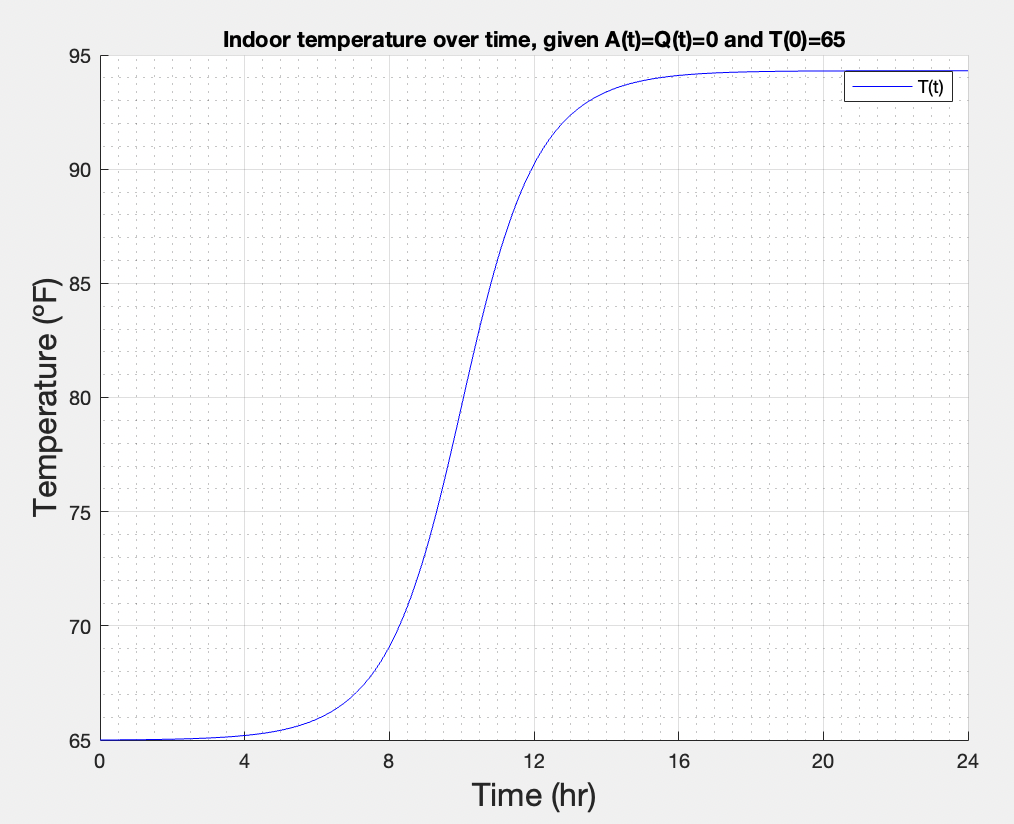
\includegraphics[width=0.4\textwidth]{./images/tempWithLights.png}}}%
    \qquad
    \subfloat[$H(t)$ given $T(0)=65\degree F$]{{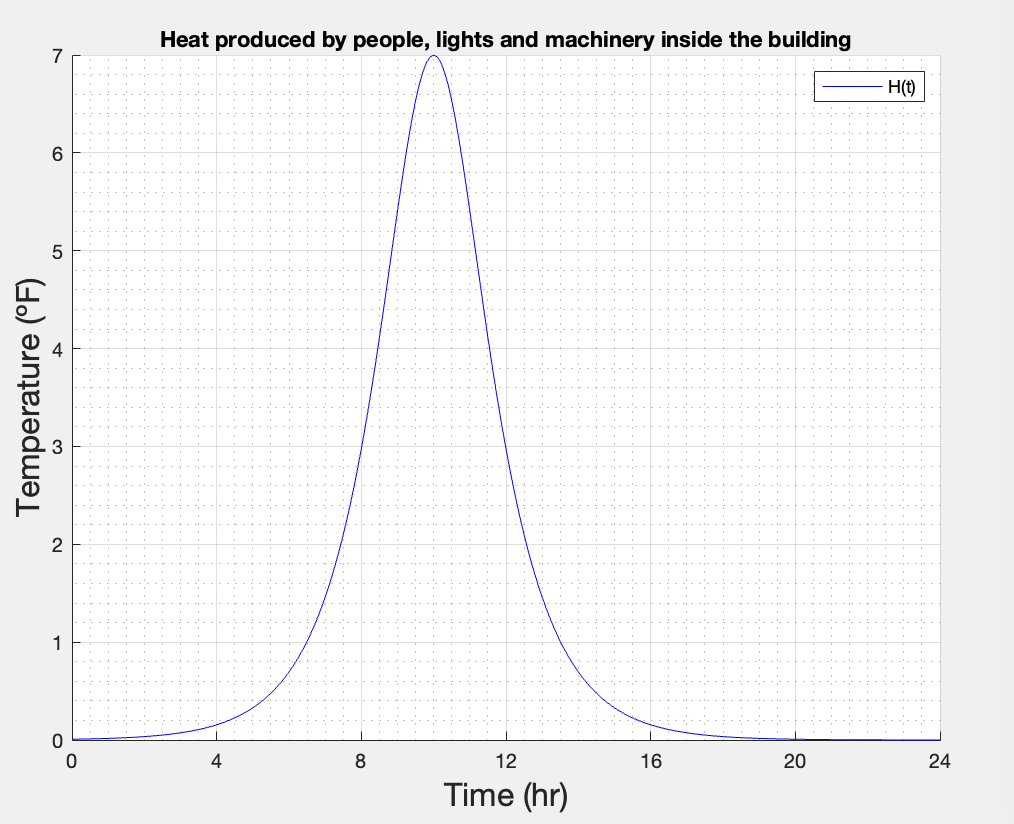
\includegraphics[width=0.4\textwidth]{./images/lights.png}}}%
    \caption{}%
    \label{fig:lights}%
\end{figure}
Now that we have these plots, let us examine some of the information that they present.
Quantitatively, from Fig.\ref{fig:lights}.a the maximum indoor temperature ($T_{max}$) occurs at $24$ hours 
and $0$ minutes, with a temperature of $94.31\degree F$. This is rather straightforward.

Qualitatively however, things are more interesting. For one, we know that $H(t)$ measures the heat produced
by people, lights, and machinery in the building, so it seems as though we could also interpret $H(t)$
as the "busyness" of the building (in others words a measure of activity). This would line up with the graph since
buildings tend to be busiest in the middle of the workday and least busy in the early morning and the late night, 
which is reflected in Fig. \ref{fig:lights}.b.

In addition, at first glance it may appear strange that $T(t)$ rises sharply in the middle of the day and then stays hot (Fig. \ref{fig:lights}.a).
However, since $H(t)$ is the only thing affecting the indoor temperature, it makes sense that $T(t)$ starts at 0, rises as the activity in the building increases, and then 
stays high as the activity dies down because there is no way for the building to lose heat. In other words, $H(t)>0$ for all $t$, 
so $\frac{dT}{dt}$ can never be negative and causes a reduction in the heat of the building.


%%%%%%%%%%%%%%%%%%%%%%%%%%%%%%%%%%%%%%%%%%%%%%%%%%%%%%%%%%%%%%%%%%%%%%%%%%%%%%%%
\section{The Effect of Furnaces and Air Conditioners} \label{furnaces and aircon}
Now we can look at the effects of furnaces and air conditioners, $Q(t)$.
Let us suppose that the thermostat is set to a constant temperature $T_d$, which is the
desired indoor temperature. The furnace and air conditioner will work together to move the indoor temperature 
to the desired temperature. Thus, we will assume that the amount of heat regulation (heating or cooling)
provided by the furnaces and the air conditioners is proportional to the difference between
the indoor temperature, $T(t)$, and the thermostat temperature, $T_d$. Consquently, we can model this behavior using:
\begin{equation}\label{eq:Q(t)}
    Q(t) = \kappa_d(T_d-T)
\end{equation}
where $\kappa_d$ is a constant of proportionality. Note that $Q(t)$ is technically a composite function
$Q([T(t)])$ which is why we considered that special case in Section \ref{Linear T(t)}. 

Now let us analyze a situation in which solely furnaces and air conditioners affect the temperature in the building, meaning $A(t)=H(t)=0$
Substituting Eq. \ref{eq:Q(t)} into Eq. \ref{T_general} subject to the assumptions above then leads to the following differential equation for this situtation.
\begin{equation} \label{eq:furnaces}
    \frac{dT}{dt} = \kappa_d(T_d-T)
\end{equation}
Let us examine a graph of some solutions to get a better understand of this equations meaning.
\begin{figure}[H]
    \centering
    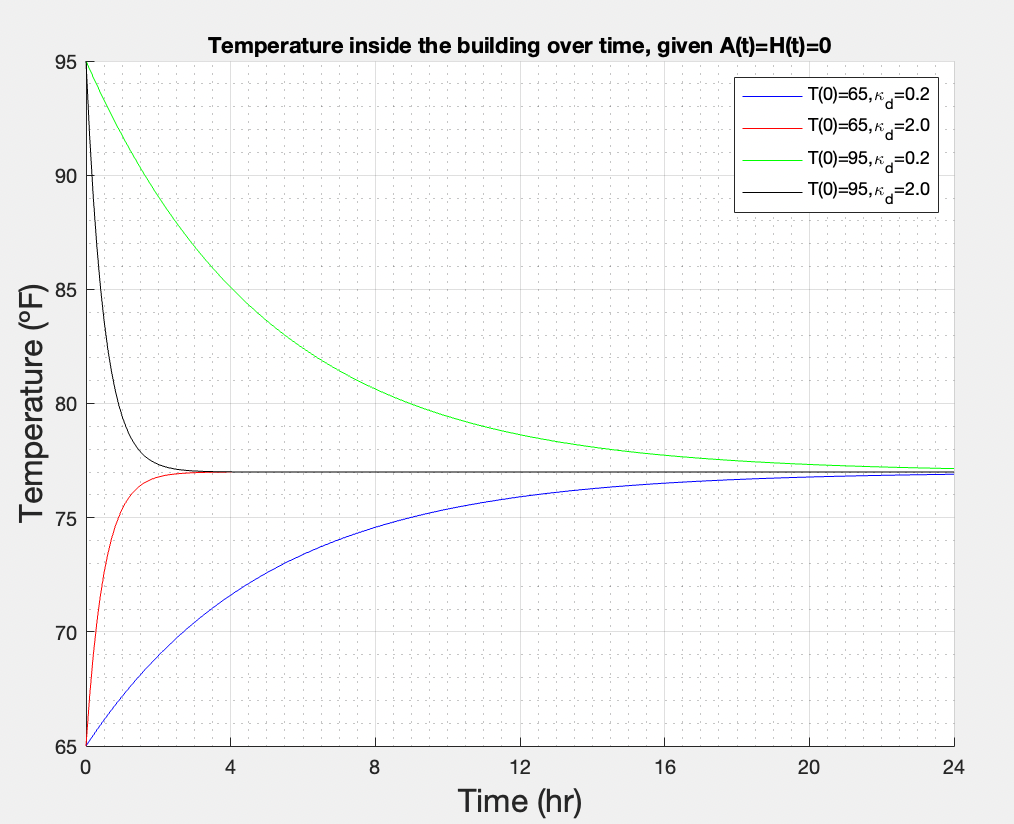
\includegraphics[width=0.6\textwidth]{./images/furnaces.png}
    \caption{Solutions to Eq. \eqref{eq:furnaces} given that $T_d=77\degree F$ with different $T_0$ and $\kappa_d$}
    \label{fig:furnaces}
\end{figure}
We can see from Fig. \ref{fig:furnaces} that the indoor temperature will eventually stabilize at $77\degree F$ which makes
sense since that is the temperature the thermostat is trying to maintain. In addition, it appears that the larger $\kappa_d$ is,
the faster the indoor temperature converges to $T_d$. This seems to suggest that $\kappa_d$ 
might stand for the quality of the temperature regulation appliances, since better furnaces and air conditioners
would regulate the temperature faster.



%%%%%%%%%%%%%%%%%%%%%%%%%%%%%%%%%%%%%%%%%%%%%%%%%%%%%%%%%%%%%%%%%%%%%%%%%%%%%%%%
\section{Analyzing the Combined Effects}
As we have discussed the effects of each of the variables seperately, we can finally
explore how combinations of them affect the indoor temperature. In particular, 
we will assume that our equipment will be damaged if the indoor temperature
exceeds $81\degree F$ and see how various combinations protect or hurt our equipment. \\ \\
Note: we will assume that $T(0)=75\degree F$ in all cases for easier comparison.

%%%%%%%%%%%%%%%%%%%%%%%%%%%%%%%%%%%%%%%%%%%%%%%%%%%%%%%%%%%%%%%%%%%%%%%%%%%%%%%%
\subsection{People, Lights, and Machinery, and Temperature Regulation}
Let us first consider a normal workday in which both $H(t)$ and $Q(t)$ affect our indoor temperature, 
giving us the following inital value problem:
\begin{equation}\label{eq:H(t) and Q(T)}
    \frac{dT}{dt} = 7\sech\left[\frac{3}{4}(t-10)\right] + 2(77-T), \qquad T(0)=75\degree F
\end{equation}
where $T_d=77\degree F$ and $\kappa_d=2$. If we examine the solution to IVP \ref{eq:H(t) and Q(T)}, 
as shown in Fig. \ref{fig:H(t) and Q(t)}, we see that the maximum indoor temperature attained occurs at 
$10$ hours and $24$ minutes, with a temperature of $80.32\degree F$. Thus, since the temperature never exceeds
$81\degree F$, this situation will prevent any harm to the equipment.
\begin{figure}[H]
    \centering
    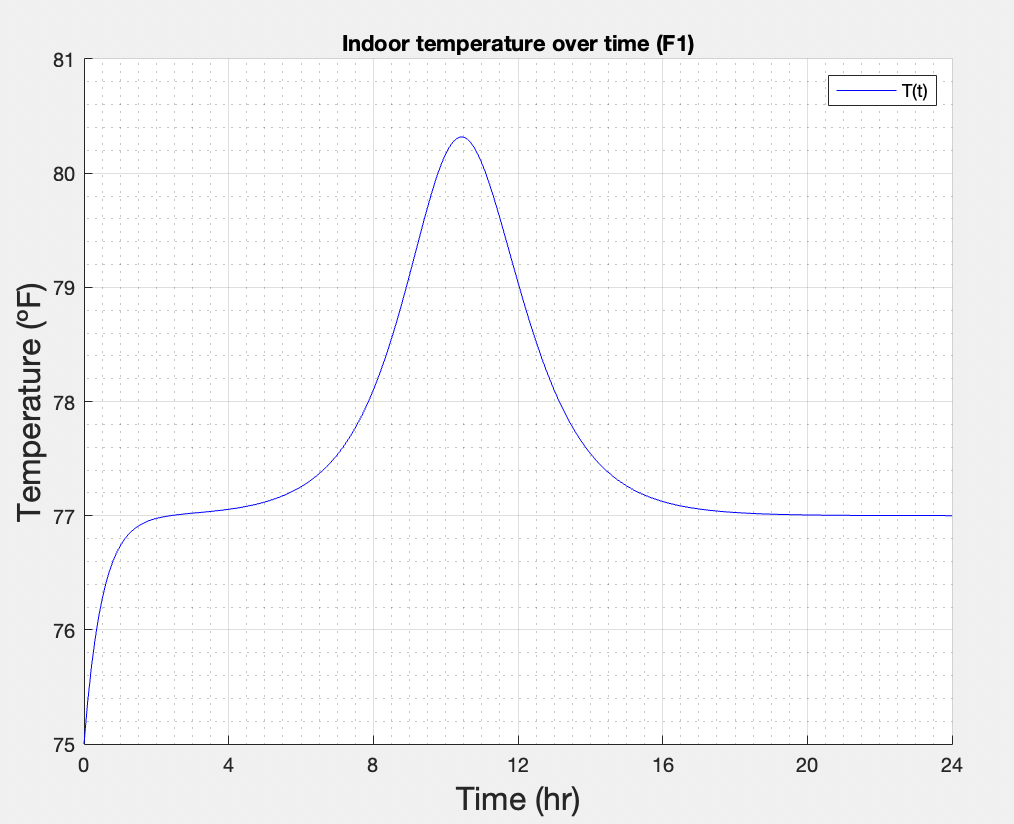
\includegraphics[width=0.6\textwidth]{./images/light_and_furnace.png}
    \caption{Solution to the IVP \eqref{eq:H(t) and Q(T)}}
    \label{fig:H(t) and Q(t)}
\end{figure}
\noindent
In addition, it is interesting to note that the air conditioning is eventually able to maintain
a consistent temperature of $77\degree F$ when activity is lower, which makes sense since that
is the $T_d$.



%%%%%%%%%%%%%%%%%%%%%%%%%%%%%%%%%%%%%%%%%%%%%%%%%%%%%%%%%%%%%%%%%%%%%%%%%%%%%%%%
\subsection{Ambient Temperature with Variable Outside Temperature} \label{hotweekendday}
Now let us consider a hot weekend day in which no people are in the building, the lights and
machines are off, and temperature regulation is off, meaning that $H(t)=Q(t)=0$ so only $A(t)$ has an effect.
We can model this situation using the following inital value problem:
\begin{equation}\label{eq:hotweekendday}
    \frac{dT}{dt} = 0.25\left[85 - 12\cos\left[\frac{\pi(t-5)}{12}\right]\right], \qquad T(0)=75\degree F
\end{equation}
where $\kappa=0.25$ and $M_0=85\degree F$. If we examine the solution to IVP \ref{eq:hotweekendday}
as shown in Fig. \ref{fig:hotweekendday} below, we see that the max indoor temperature reached is $91.82\degree F$ 
which occurs at $20$ hours and $6$ minutes. This of course means that equipment will be damaged since the indoor temperature
exceeds $81\degree F$, and in particular that damage will start at $12$ hours and $12$ minutes.
\begin{figure}[H]
    \centering
    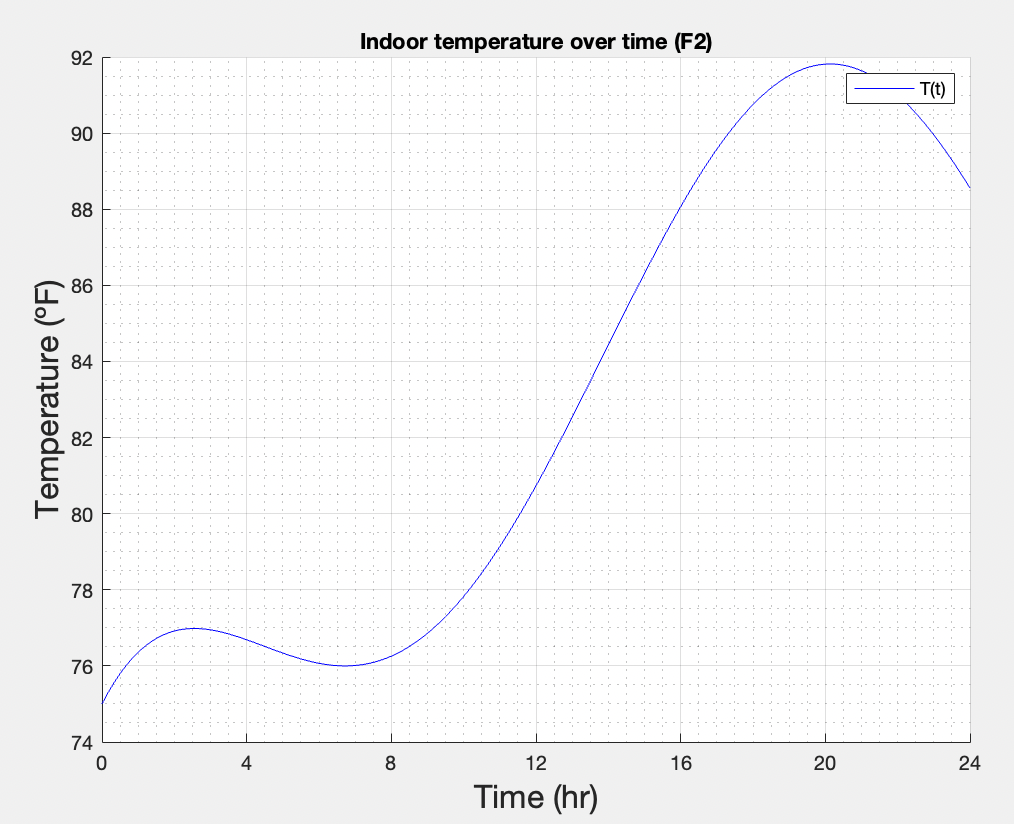
\includegraphics[width=0.6\textwidth]{./images/hotWeekendDay.png}
    \caption{Solution to the IVP \eqref{eq:hotweekendday}}
    \label{fig:hotweekendday}
\end{figure}




%%%%%%%%%%%%%%%%%%%%%%%%%%%%%%%%%%%%%%%%%%%%%%%%%%%%%%%%%%%%%%%%%%%%%%%%%%%%%%%%
\subsection{Ambient Temperature, and Furnaces and Air Conditioners}
Now we will consider the same scenario as Section \ref{hotweekendday} but we will add the effects
of air conditioners and furnaces, $Q(t)$ to see what impact they make. Thus, this situation can be modeled
using the following inital value problem
\begin{equation}\label{eq:ambient and furnace}
    \frac{dT}{dt} = 0.25\left[85 - 12\cos\left[\frac{\pi(t-5)}{12}\right]\right] + \kappa_d(77-T), \qquad T(0)=75\degree F
\end{equation}
where $\kappa=0.25$, $M_0=85\degree F$, and $T_d=77\degree F$. Let us consider two cases in which
$\kappa_d=2$ and $\kappa_d=0.5$ to further see what impact they have.
\begin{figure}[H]
    \centering
    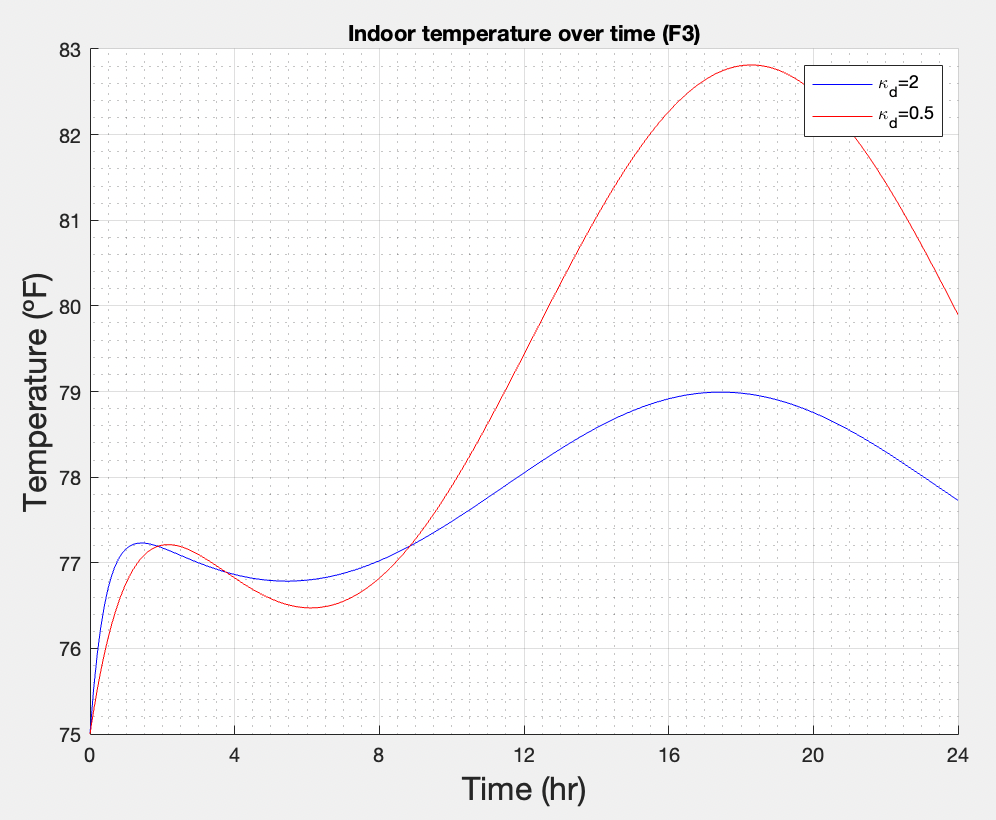
\includegraphics[width=0.6\textwidth]{./images/ambientAndFurnace.png}
    \caption{Solutions to the IVP \eqref{eq:ambient and furnace} with different $\kappa_d$}
    \label{fig:ambient and furnace}
\end{figure}
If we examine the solution to IVP \ref{eq:ambient and furnace} as shown in Fig. \ref{fig:ambient and furnace}, we see that 
when $\kappa_d=2$ the max indoor temperature reached is $78.99\degree F$ which means that the equipment will be safe.
On the other hand, when $\kappa_d=0.5$ the max indoor temperature reached is $82.81\degree F$ which means that 
the equipment will not be safe. The equipment in this case would be exposed to damaging temperatures for
$8$ hours and $36$ minutes. Either way, this proves that ambient temperature considered with
furnaces and air conditioners is safer since the max temperatures are much lower, which
aligns with our intuition.

%%%%%%%%%%%%%%%%%%%%%%%%%%%%%%%%%%%%%%%%%%%%%%%%%%%%%%%%%%%%%%%%%%%%%%%%%%%%%%%%
\subsection{The Effect of All Three Varibles}
Finally, we can now consider the combined effects of $H(t), Q(t)$
and $A(t)$ on indoor temperature. To analyze this situation in all
its complexity, let us consider a longer time range from Friday to Sunday
where employees come to work on Friday and go home Friday night,
leaving the building vacant over the weekend. We can model this situation using the following inital value problem:
\begin{equation}\label{eq:all together now}
    \frac{dT}{dt} = 0.25\left[85 - 12\cos\left[\frac{\pi(t-5)}{12}\right]\right] + 7\sech\left[\frac{3}{4}(t-10)\right] +  2(77-T), \qquad T(0)=75\degree F
\end{equation}
You will notice that we have now come full circle, as Eq. \eqref{eq:all together now} is the functional, filled-in form of our initial temperature model
Eq. \eqref{T_general}, with $\kappa=0.25$, $M_0=85\degree F$,$\kappa_d=2$ and $T_d=77\degree F$. Let us now examine the solution to this
IVP.
\begin{figure}[H]
    \centering
    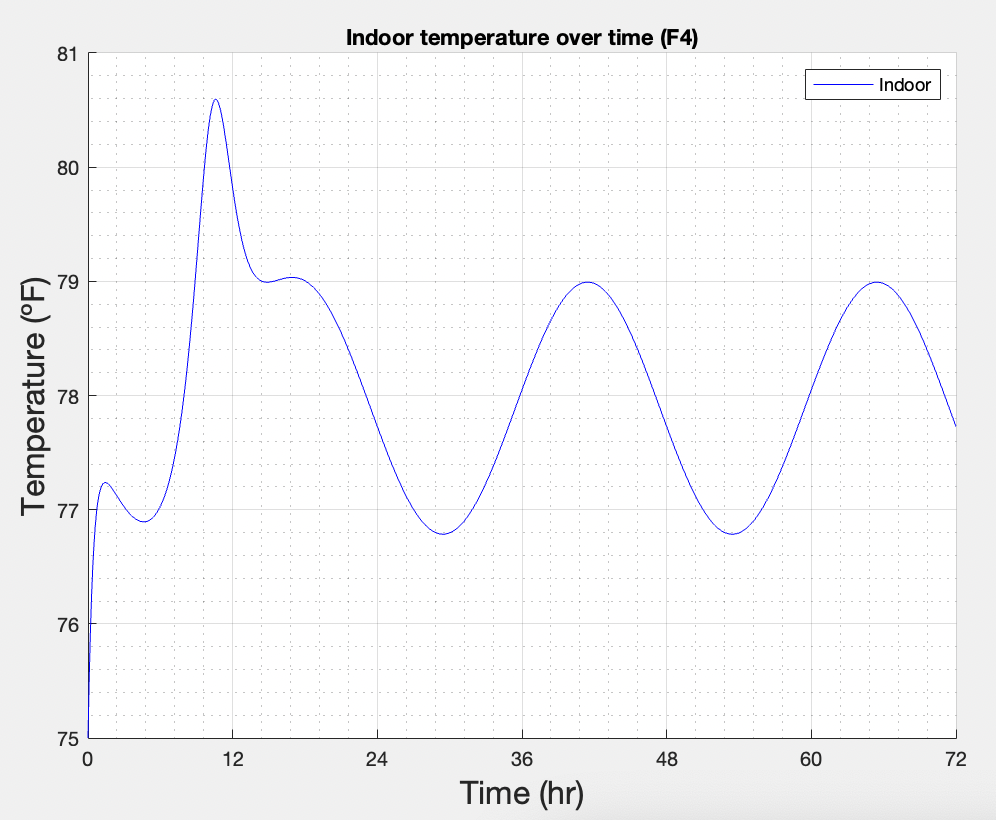
\includegraphics[width=0.6\textwidth]{./images/allTogetherNow.png}
    \caption{Solution to IVP \eqref{eq:all together now} using $720$ points}
    \label{fig:all together now}
\end{figure}
As we can see from the solution shown in Fig. \ref{fig:all together now}, the indoor temperature for the combined situation
never surpasses $81\degree F$ which means that the equipment would be safe the entire time. In addition, it appears as 
the solution seems to reach a "steady state" beginning around $30$ hours where it is in a consistent oscillatory state.
Looking at Eq. \eqref{eq:all together now}, this "steady state" seems to come from the outside ambient temperature term, 
specifically the $\cos()$ within it.

To verify this idea, let us inspect that term, mainly:
\begin{equation}\label{eq:specificM}
    M(t) = 85 - 12\cos\left[\frac{\pi(t-5)}{12}\right]
\end{equation}
Looking at Fig. \ref{fig:specificM} below, we see steady state osscilatory behavior, similar to that found in
Fig. \ref{eq:all together now}, just with larger amplitudes. Thus, it would appear our suspicion was correct
in that the outside ambient temperature is driving the steady state behavior for the temperature inside the building 
during the weekend.

Using these facts to inform us, we can thus put forward and explanation for the entirety of the solution for
Eq. \eqref{eq:all together now}. When Friday starts, the building is cool, and as the 
activity inside the building grows, the air conditioning and the heating do their best to keep up.
However the air conditioning is no match for peak activity heat combined with the midday heat,
so we see a spike in heat midday  on Friday. Then, as activity and ambient temperature reduce, keeping
in mind the activity does not pick back up, the temperature settles into a steady cycle for the rest of the
weekend as the ambient temperature and the air conditioners and furnaces go back and forth.

\begin{figure}[H]
    \centering
    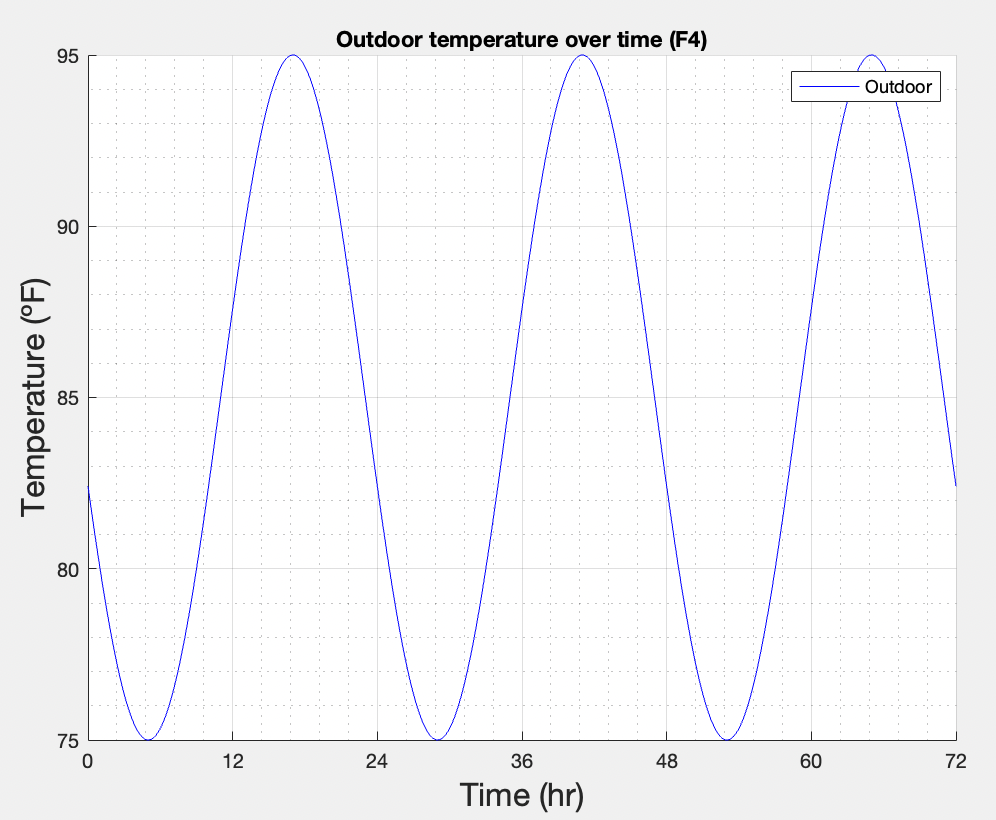
\includegraphics[width=0.6\textwidth]{./images/specificM.png}
    \caption{Plot of M(t) [Eq. \eqref{eq:specificM}] over time}
    \label{fig:specificM}
\end{figure}


%%%%%%%%%%%%%%%%%%%%%%%%%%%%%%%%%%%%%%%%%%%%%%%%%%%%%%%%%%%%%%%%%%%%%%%%%%%%%%%
\section{Conclusion}
In this project, we modeled the temperature in a building considering the ambient temperature outside, the heat produced by humans, lights, and machines, and heating and cooling appliances.
We found that when all factors are eliminated except the impact of ambient temperature on the temperature inside the building, the temperature trends towards the outside temperature. 
When considering just the heat produced by humans, lights, and machines, the indoor temperature rises when there is activity in the building, and when all the activity ends, it maintains a steady high temperature.
When only the heating and cooling appliances are used with no other variables considered, the temperature in the building trends toward the desired temperature, maintaining at the desired temperature afterwards. 
We found that when you combine all three of these factors together, your model reflects each element simultaneously. The temperature rises higher during the weekdays due to the influx of people and the rising temperature outside. 
On the weekends, the temperature then begins to fluctuate in a steady oscillating pattern, not reaching as high as the weekdays without the flow of people.


%%%%%%%%%%%%%%%%%%%%%%%%%%%%%%%%%%%%%%%%%%%%%%%%%%%%%%%%%%%%%%%%%%%%%%%%%%%%%%%%
\newpage
\section{Appendix}

\subsection{Calculations}
\subsubsection{General Solution of $T(t)$ Using Integating Factors}\label{calc:integrating factors}
\begin{align*}
    \frac{dT}{dt} &= \kappa[M(t)-T(t)]+H(t)+Q(t) \\
    \frac{dT}{dt} &= \kappa M(t)- \kappa T(t) +H(t)+Q(t) \\
    \frac{dT}{dt} + \kappa T(t) &= \kappa M(t) +H(t)+Q(t) \\
    \mu &= e^{\int \:\kappa dt} \tag{integrating factor}\\
    \mu &= e^{\kappa t} \\
    (e^{\kappa t} T)' &= [\kappa M(t)+H(t)+Q(t)]e^{\kappa t} \\
    \text{let } y(t) &=e^{\kappa t} T(t) \tag{substitution}\\
    y'(t) &= [\kappa M(t)+H(t)+Q(t)]e^{\kappa t} \\
    \int _{t_0}^t\:y'\left(s\right)ds &= \int _{t_0}^t\:[\kappa[M(s)-T(s)]+H(s)+Q(s)]e^{\kappa s}ds\\
    y(t)-y(t_0) &= \int _{t_0}^t\:[\kappa M(s)+H(s)+Q(s)]e^{\kappa s}ds\\
    y(t) &= \int _{t_0}^t\:[\kappa M(s)+H(s)+Q(s)]e^{\kappa s}ds +y(t_0)\\
    e^{\kappa t} T(t) &= \int _{t_0}^t\:[\kappa M(s)+H(s)+Q(s)]e^{\kappa s}ds +e^{\kappa t_0} T(t_0)\\
    T(t) &= e^{-\kappa t}\int _{t_0}^t\:[\kappa M(s)+H(s)+Q(s)]e^{\kappa s}ds +e^{\kappa (t_0-t)} T(t_0)\\
    T(t) &= e^{-\kappa t}\int _{t_0}^t\:[\kappa M(s)+H(s)+Q(s)]e^{\kappa s}ds +e^{\kappa (t_0-t)} T_0        
\end{align*}

\subsubsection{Analytical Solution to the General Solution Given Certain Assumptions}\label{calc:analytical}
%Ben make sure to state the assumptions be held here
\begin{center}
    Situation/Assumptions: $H(t)=Q(t)=0$, $M(t)=M_0$, and $T(t_0)=T_0$
\end{center}
\begin{align*}
    T(t) &= e^{-\kappa t}\int _{t_0}^t\:[\kappa M(s)+H(s)+Q(s)]e^{\kappa s}ds +e^{\kappa (t_0-t)} T_0 \tag{general solution}\\
    T(t) &= e^{-\kappa t}\int _{t_0}^t\:[\kappa M_0]e^{\kappa s}ds +e^{\kappa (t_0-t)} T_0 \tag{plug in assumptions}\\
    T(t) &= e^{-\kappa t} M_0 e^{\kappa s}|_{s=t_0}^s=t\: +e^{\kappa (t_0-t)} T_0\\
    T(t) &= e^{-\kappa t} M_0 (e^{\kappa t}-e^{\kappa t_0})  +e^{\kappa (t_0-t)} T_0\\
    T(t) &= M_0 - M_0 e^{\kappa (t_0-t)}  +e^{\kappa (t_0-t)} T_0\\
    T(t) &= M_0 + (T_0 - M_0 e^{\kappa (t_0-t)}) 
\end{align*}

\subsubsection{Time Constant Calculation}\label{calc:time constant}
\begin{align*}
    \Delta t &= t-t_0 \tag{definition of time constant}\\
    t &= \Delta t +t_0 
\end{align*}
\begin{center}
    Find the value of time constant when the difference between the building's temperature and
    the outside temperature is $e^-1$ of the initial difference.
\end{center}
\begin{align*}
 e^{-1}(T_0-M_0)&= T(t)-M(t) \\
 e^{-1}(T_0-M_0)&= T(t)-M_0\\
 e^{-1}(T_0-M_0)&= M_0+(T_0-M_0)e^{\kappa (t_0 - t) } - M_0\\
 e^{-1}(T_0-M_0)&=(T_0-M_0)e^{\kappa (t_0 - \Delta t + t_0) } \\
 e^{-1}&=e^{\kappa (- \Delta t) } \\
 -1&=-\kappa \Delta t   \\
 \Delta t &= \frac{1}{\kappa}
\end{align*}
\subsection{Code}
\subsubsection{Runge-Kutta Fourth Order Method (Task Set B)}\label{Runge-Kutta}
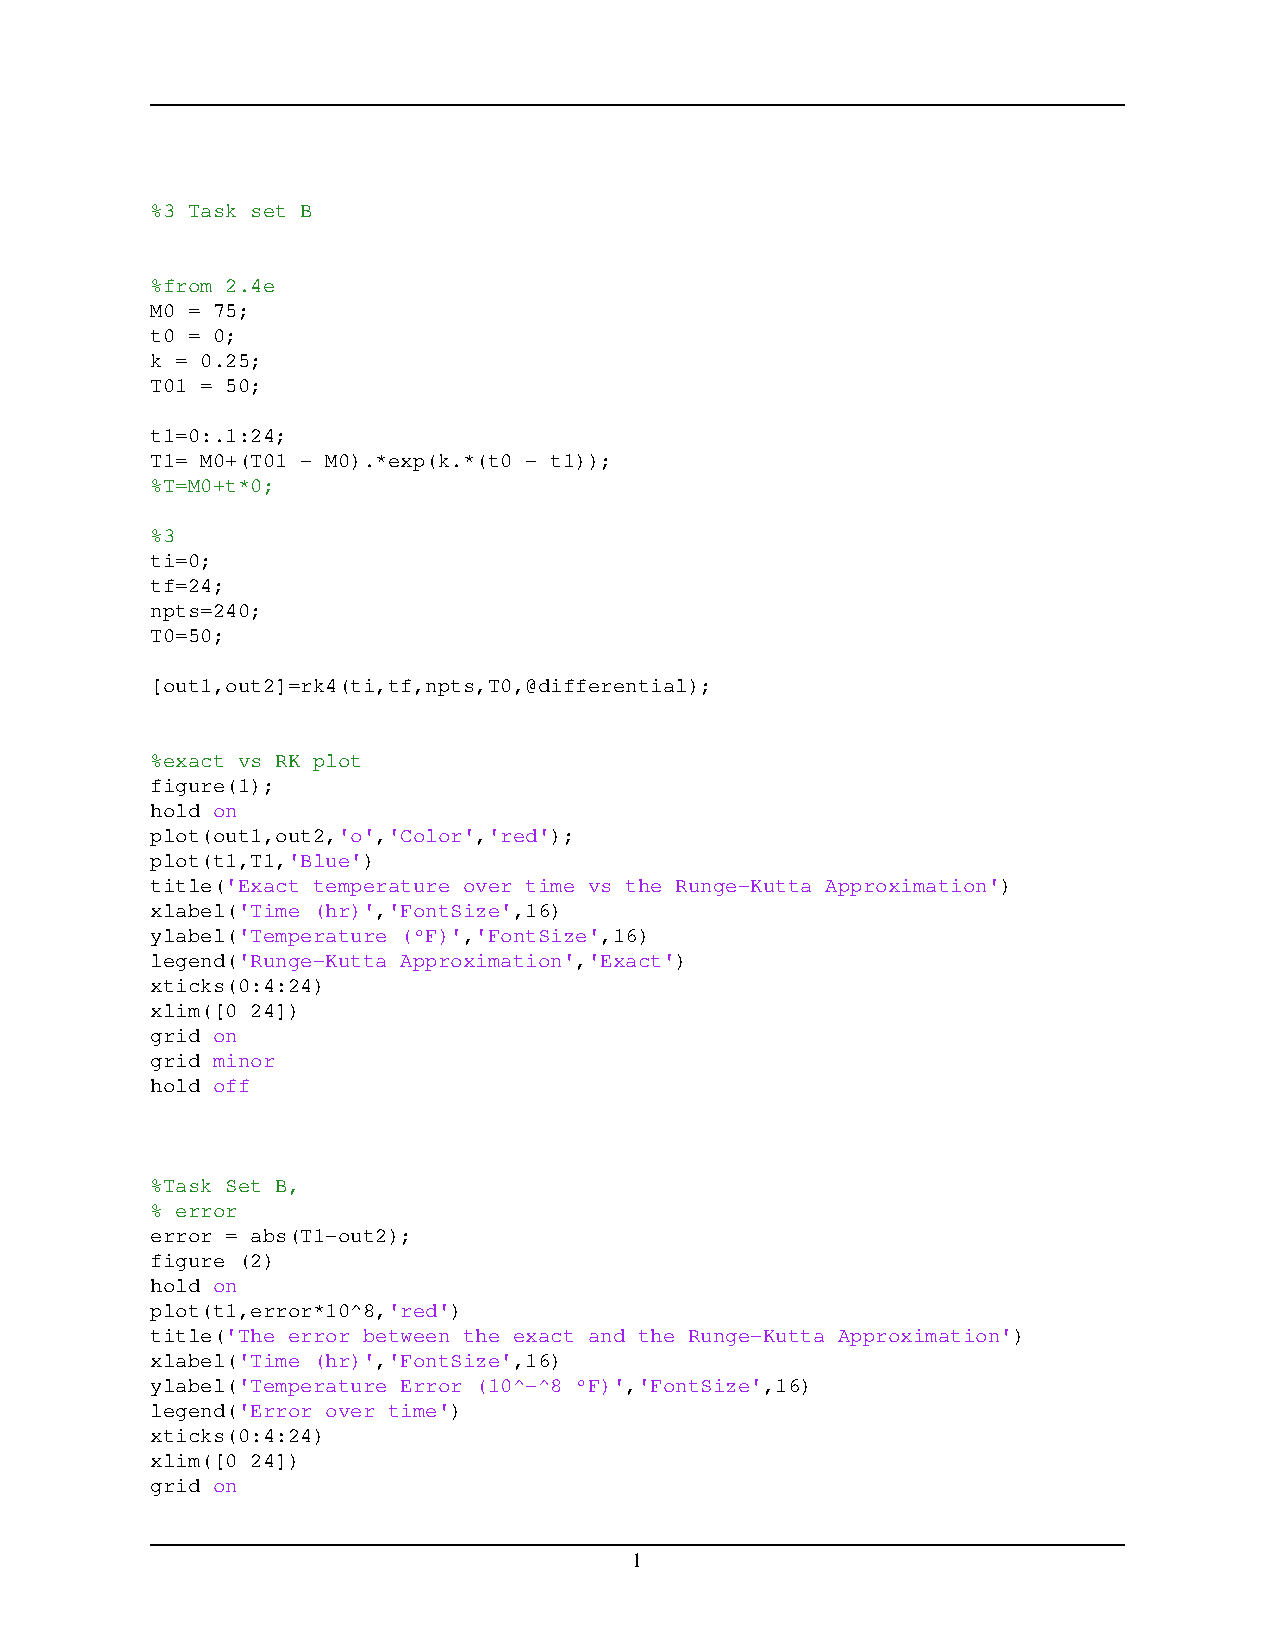
\includepdf[pages=-]{./codePdfs/DEProj1part3.pdf}
\subsubsection{The Rest}
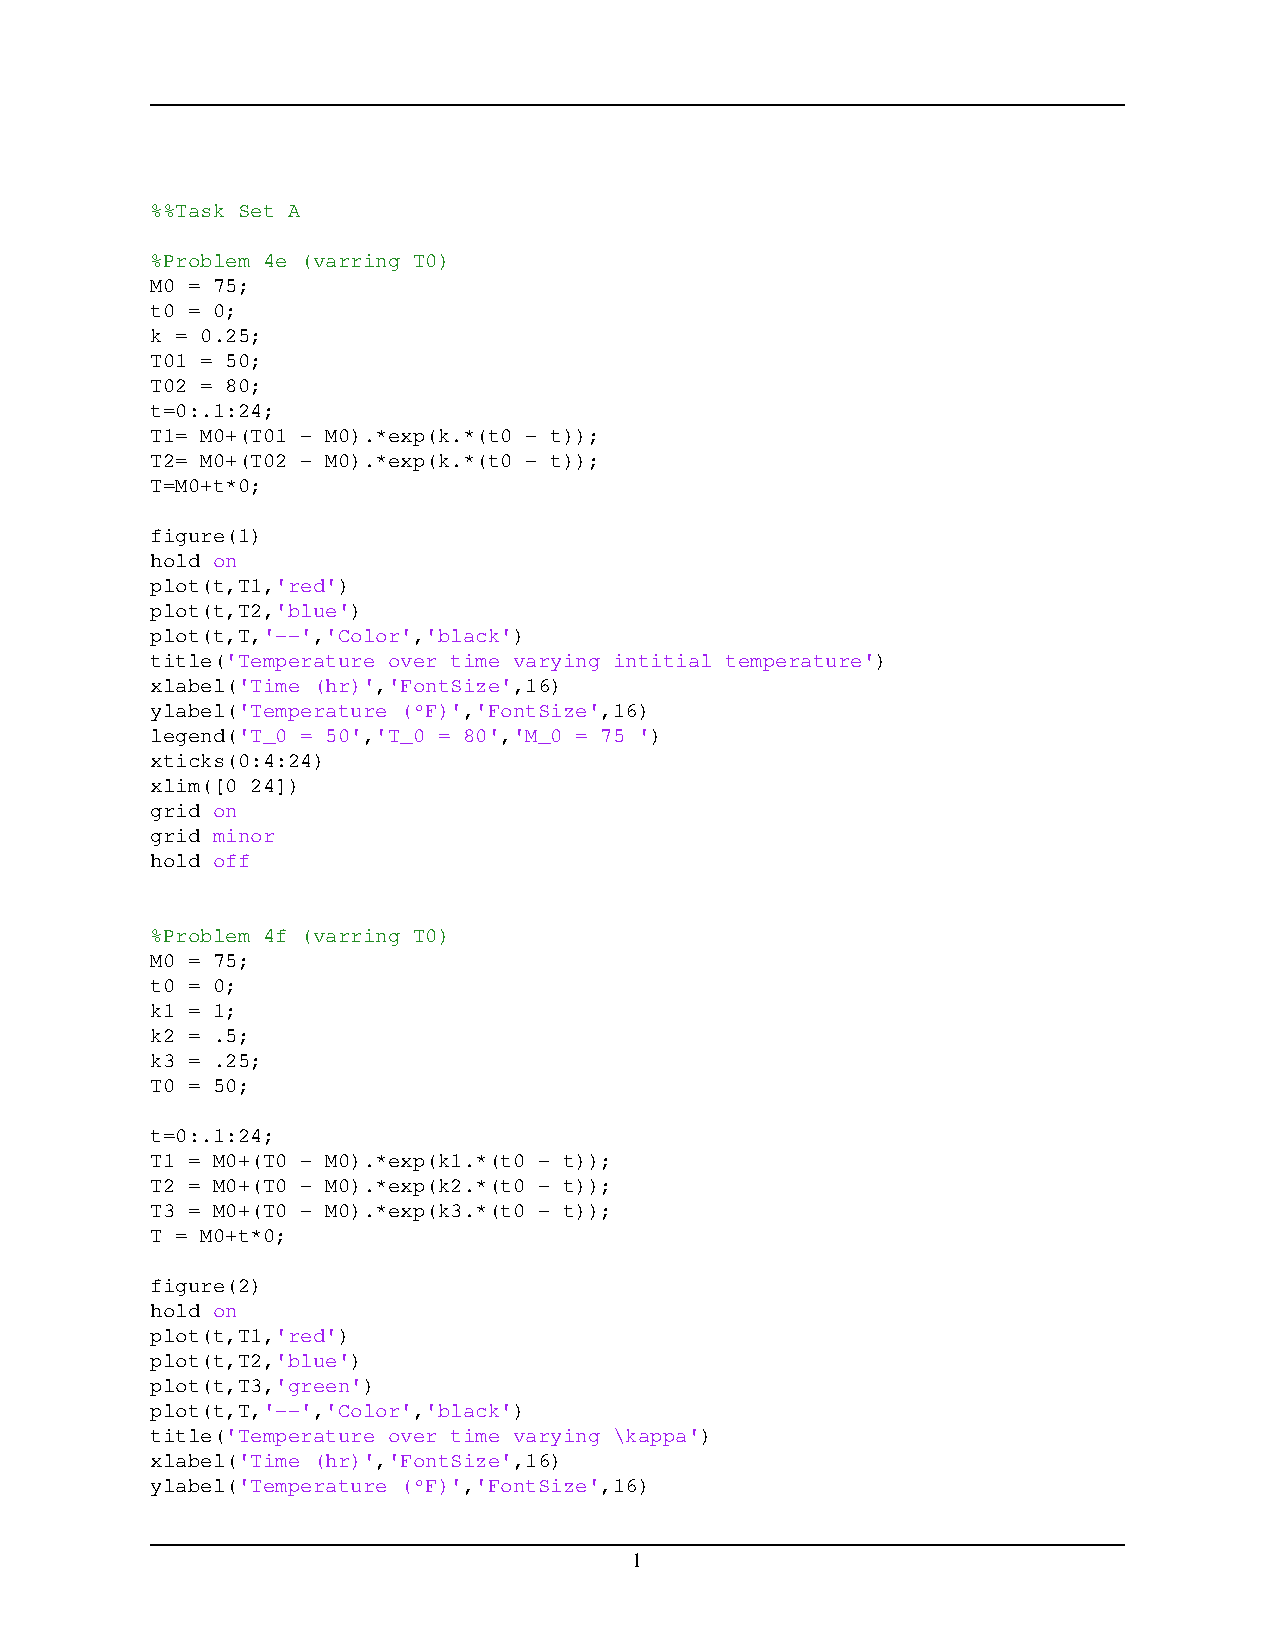
\includepdf[pages=-]{./codePdfs/DEProj1.pdf}
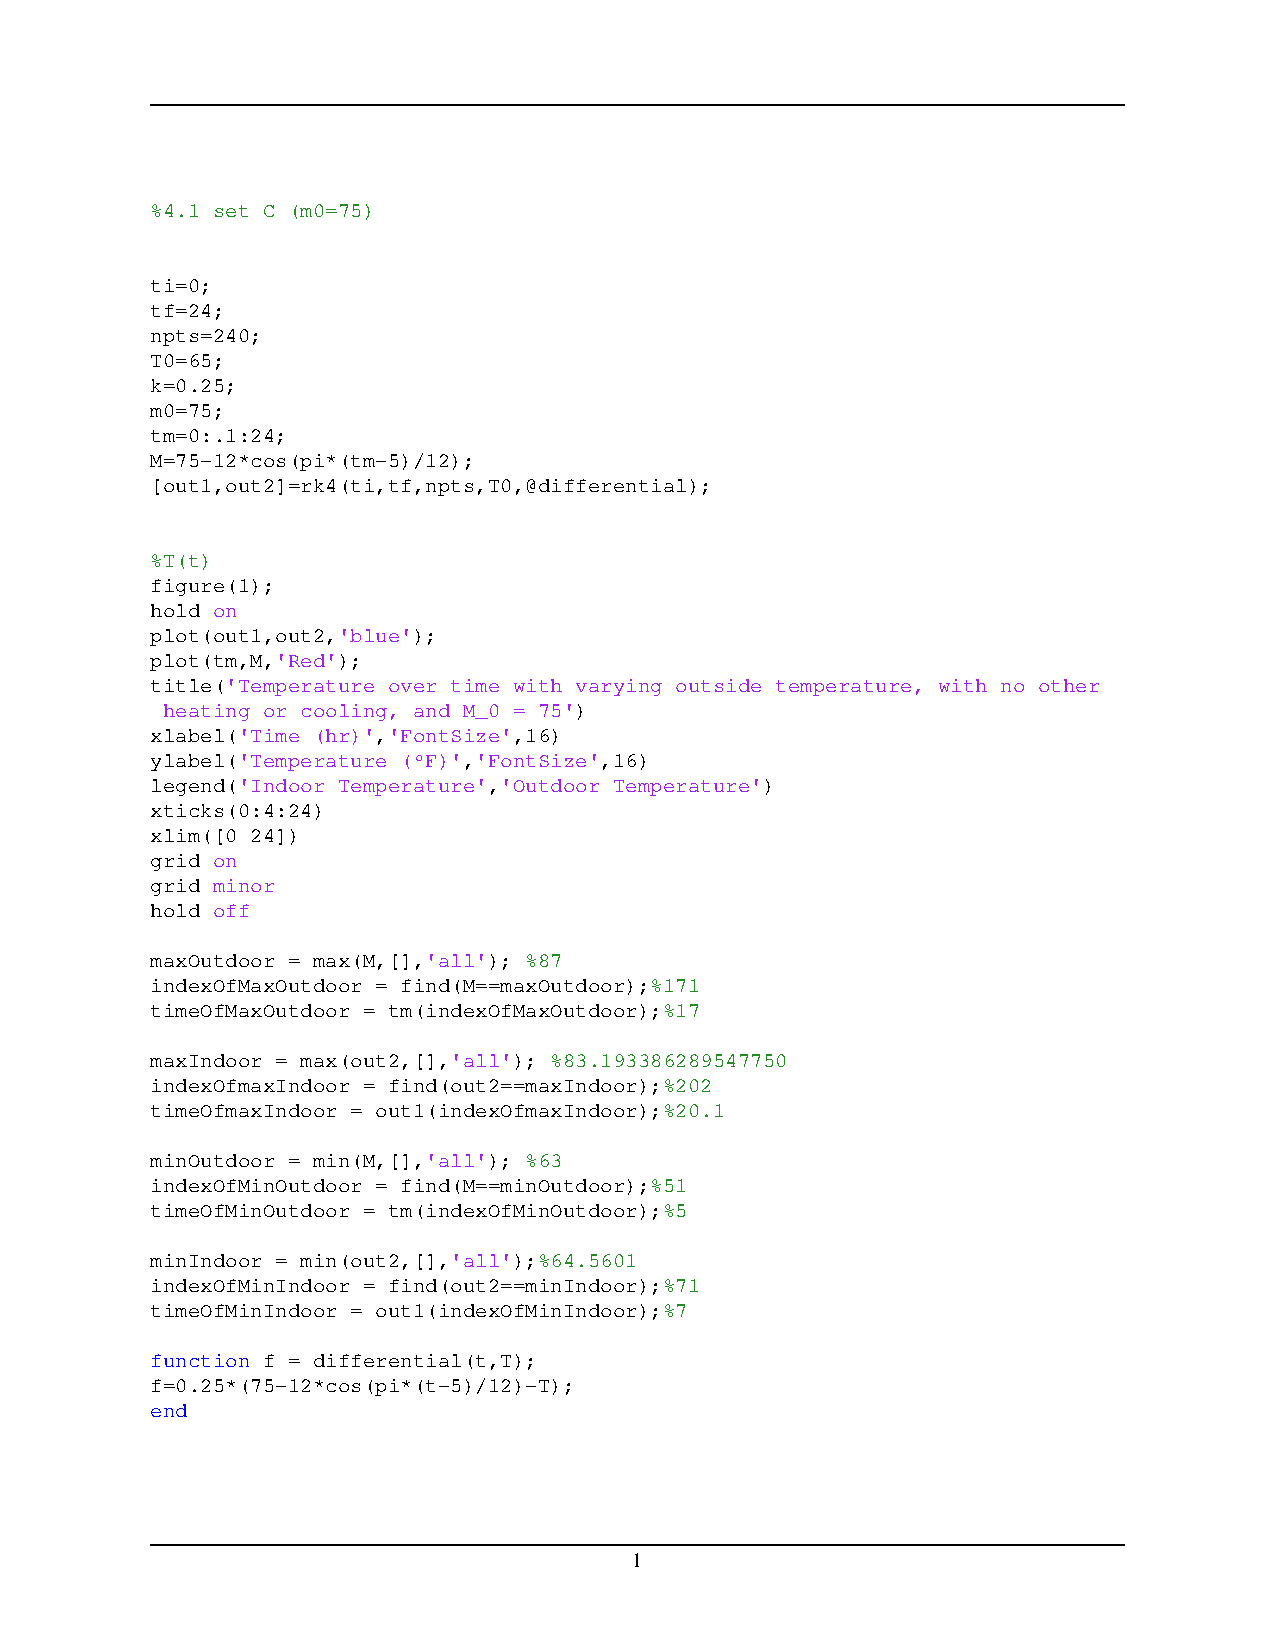
\includepdf[pages=-]{./codePdfs/DeProj1part4.pdf}
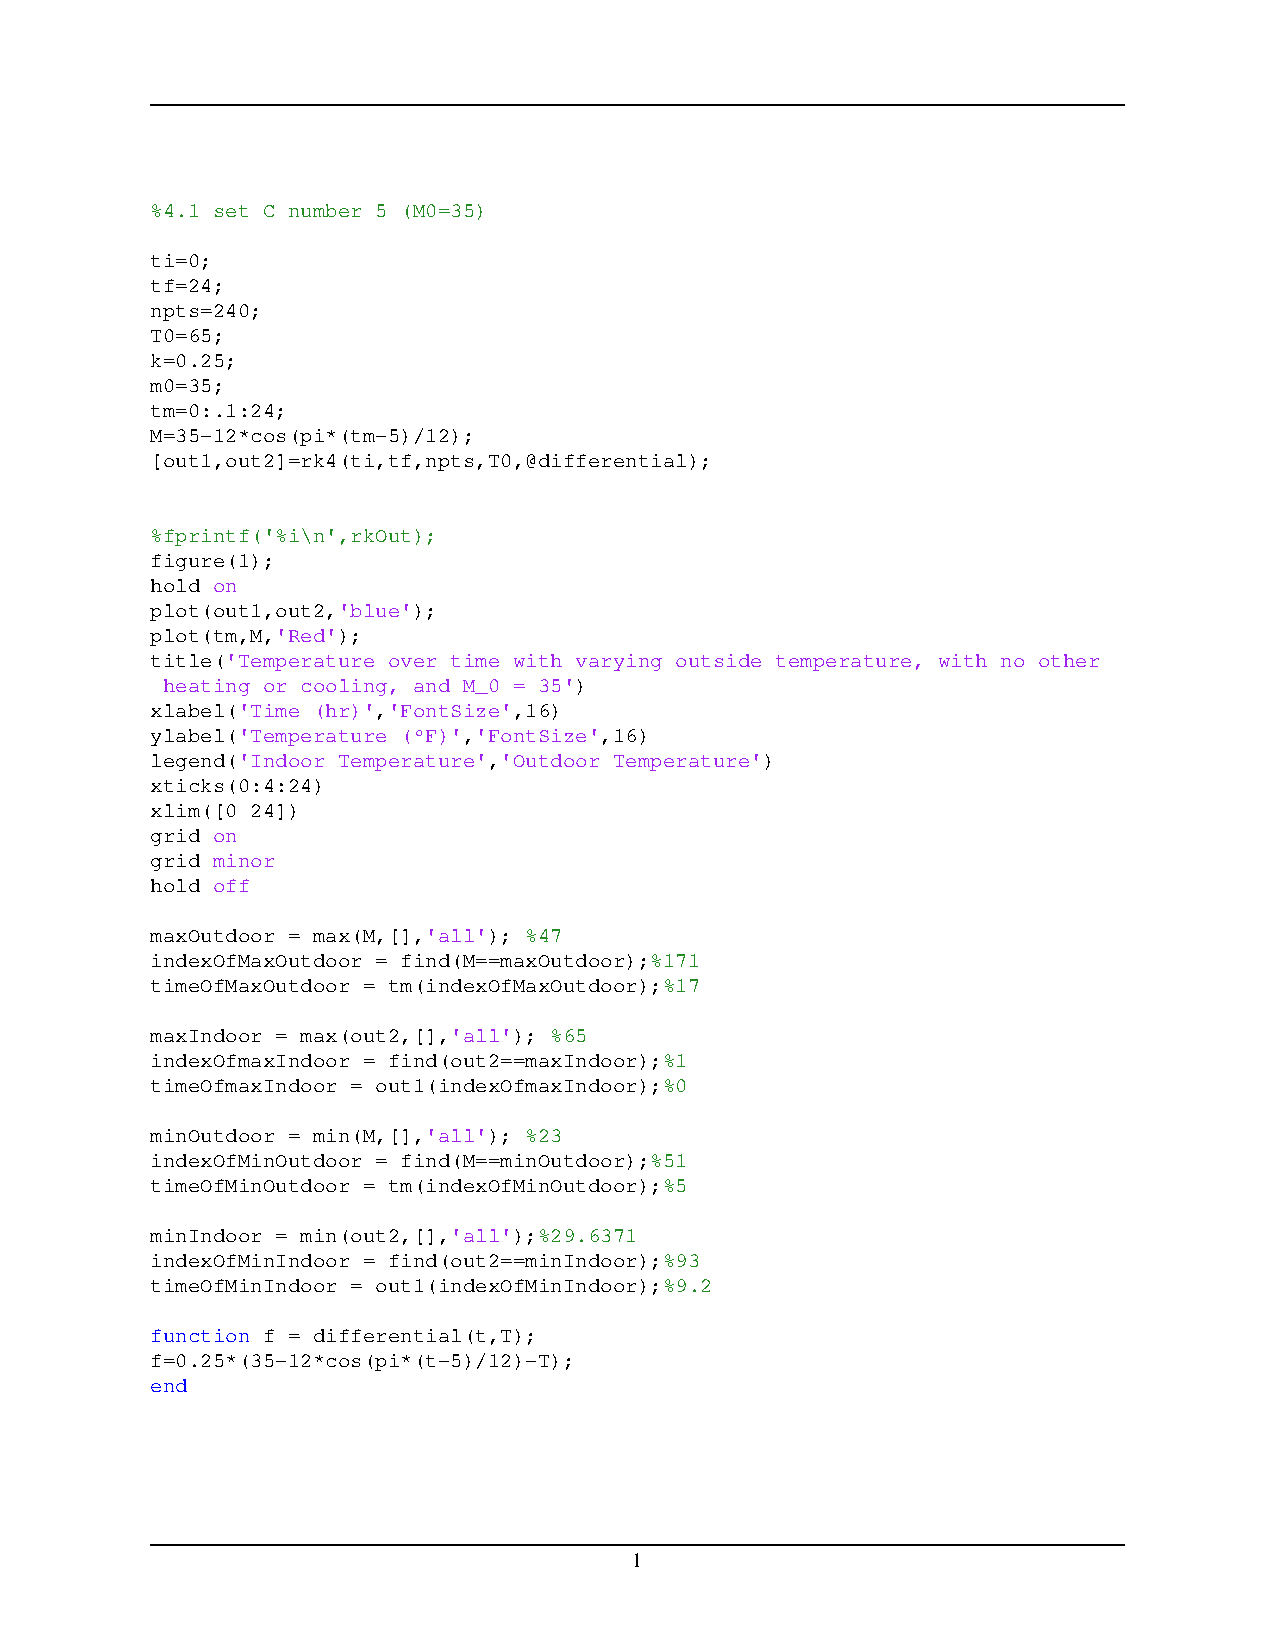
\includepdf[pages=-]{./codePdfs/dEProj1part4_1_5.pdf}
%\subsubsection{Task Set D}
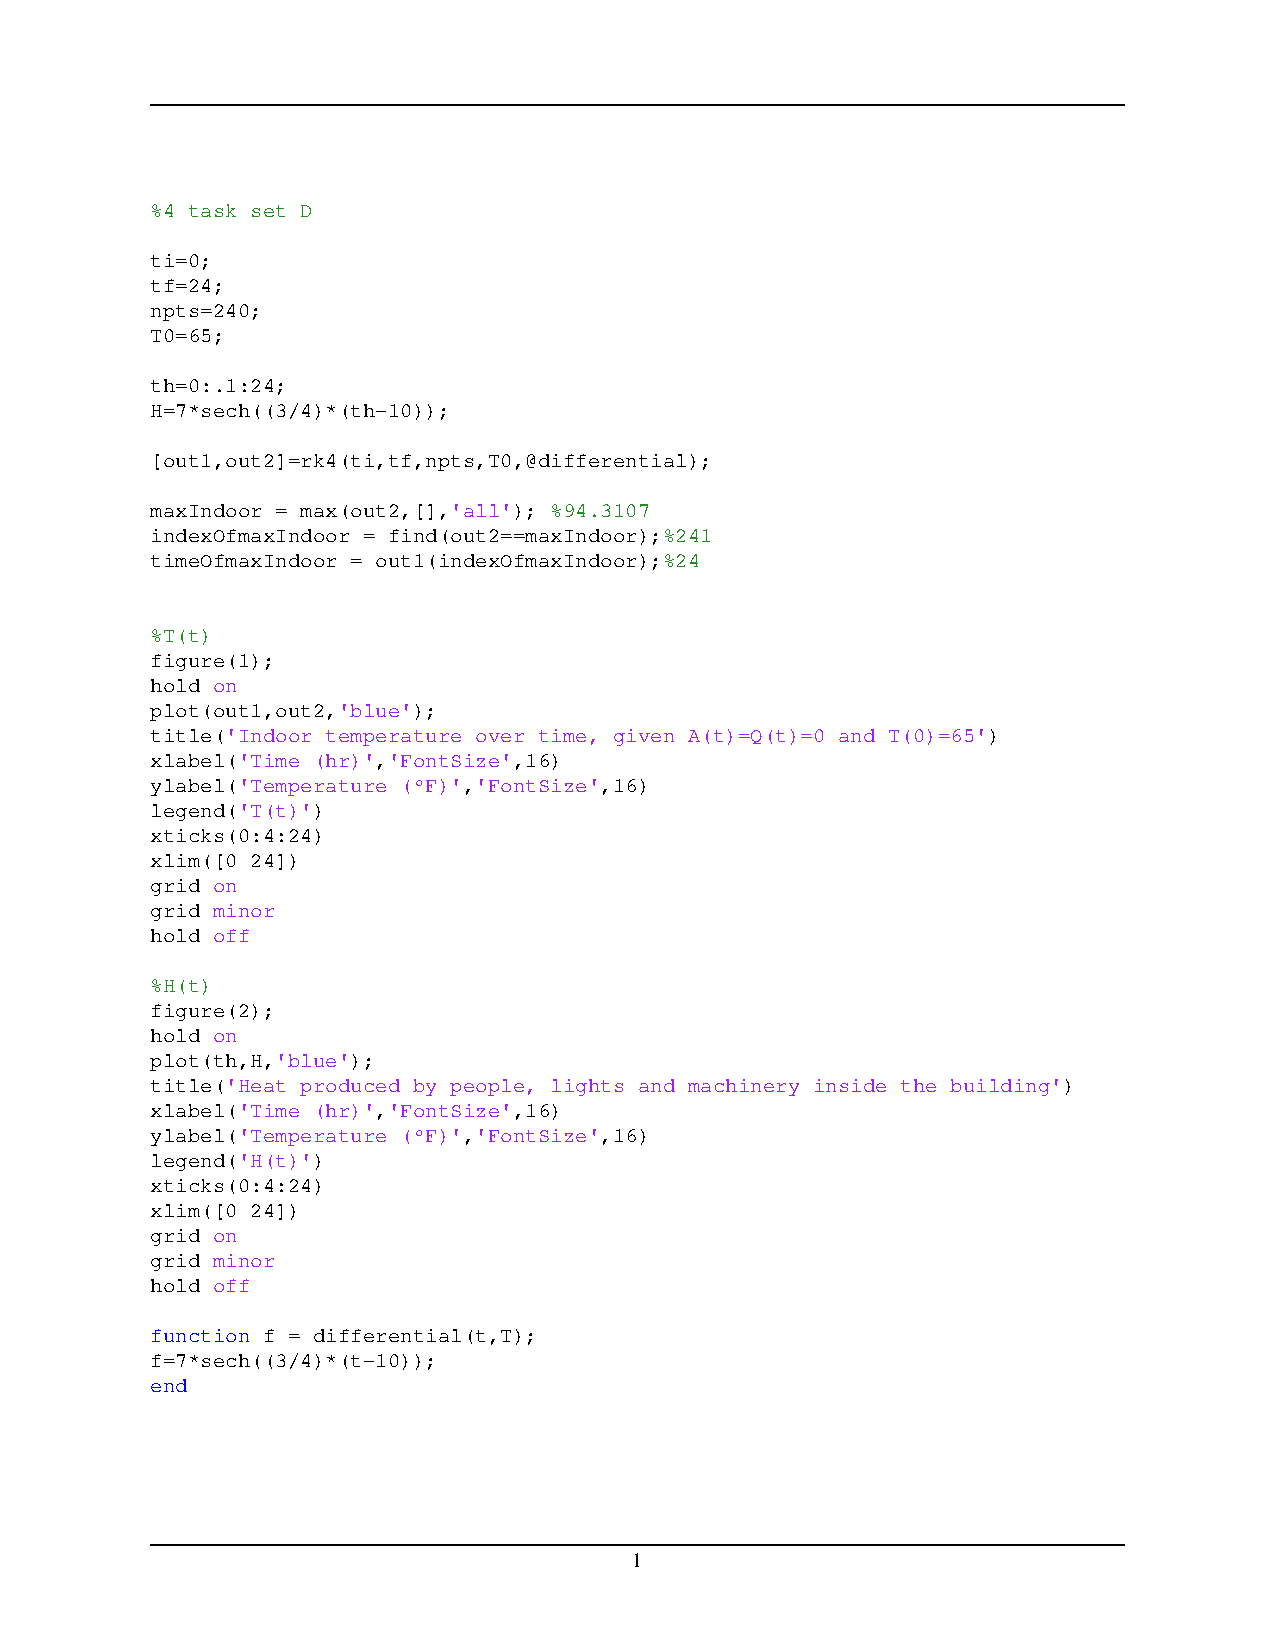
\includepdf[pages=-]{./codePdfs/Deproject4D.pdf}
%\subsubsection{Task Set E}
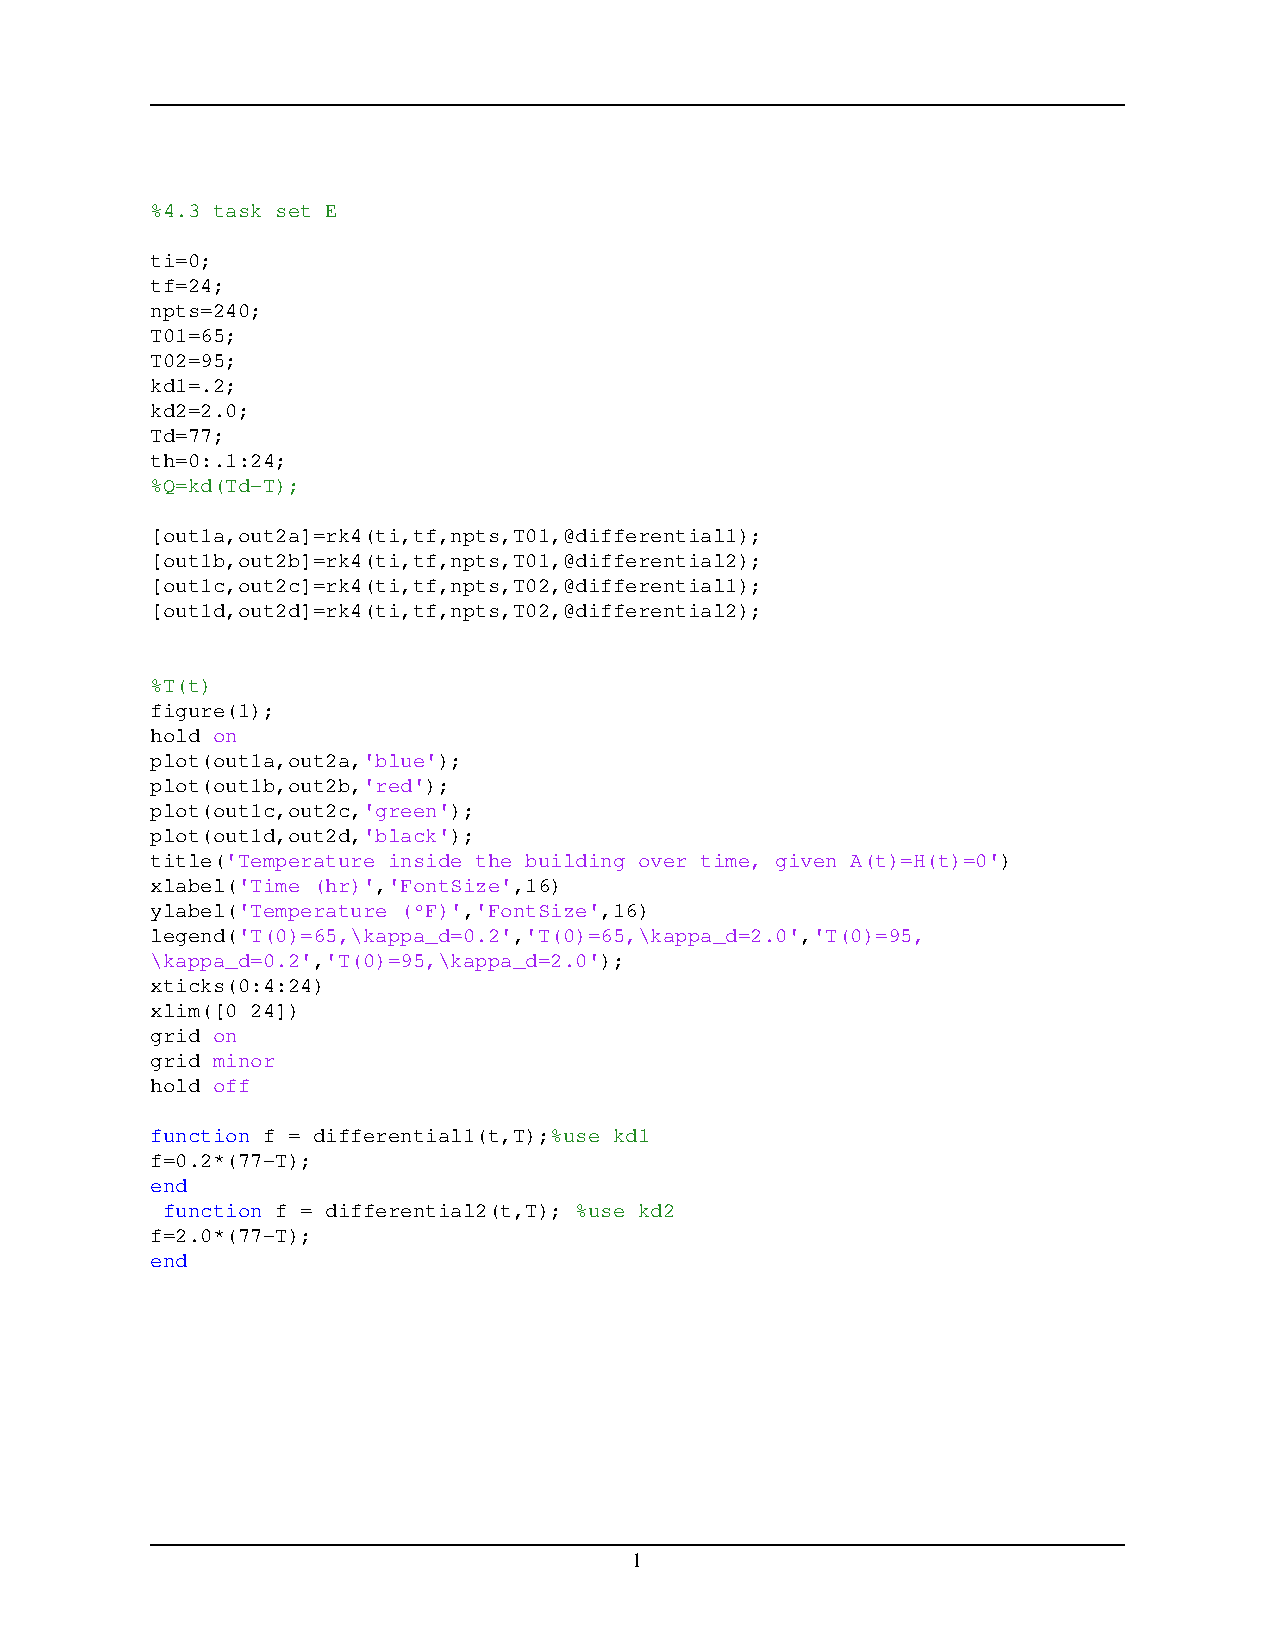
\includepdf[pages=-]{./codePdfs/DeProj1part4E.pdf}
%\subsubsection{Task Set F}
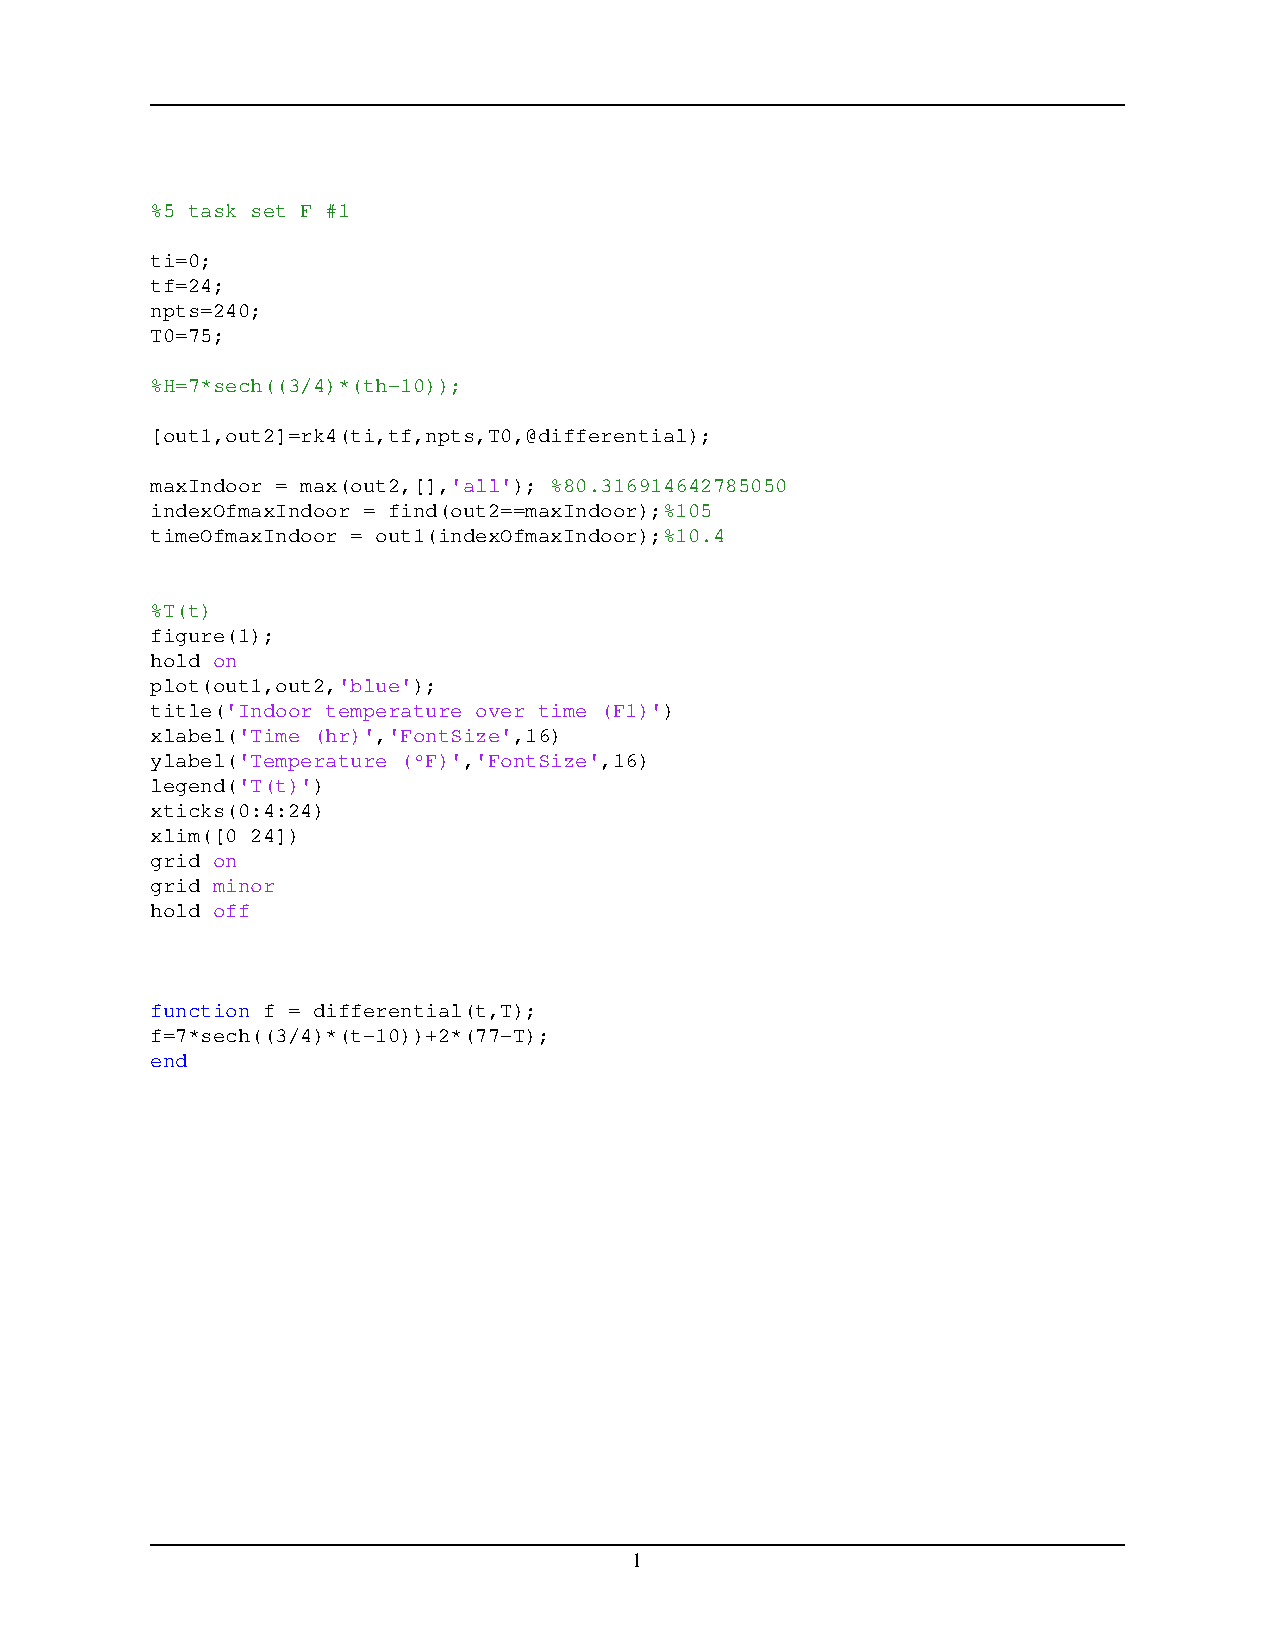
\includepdf[pages=-]{./codePdfs/DeProj1part5F1.pdf}
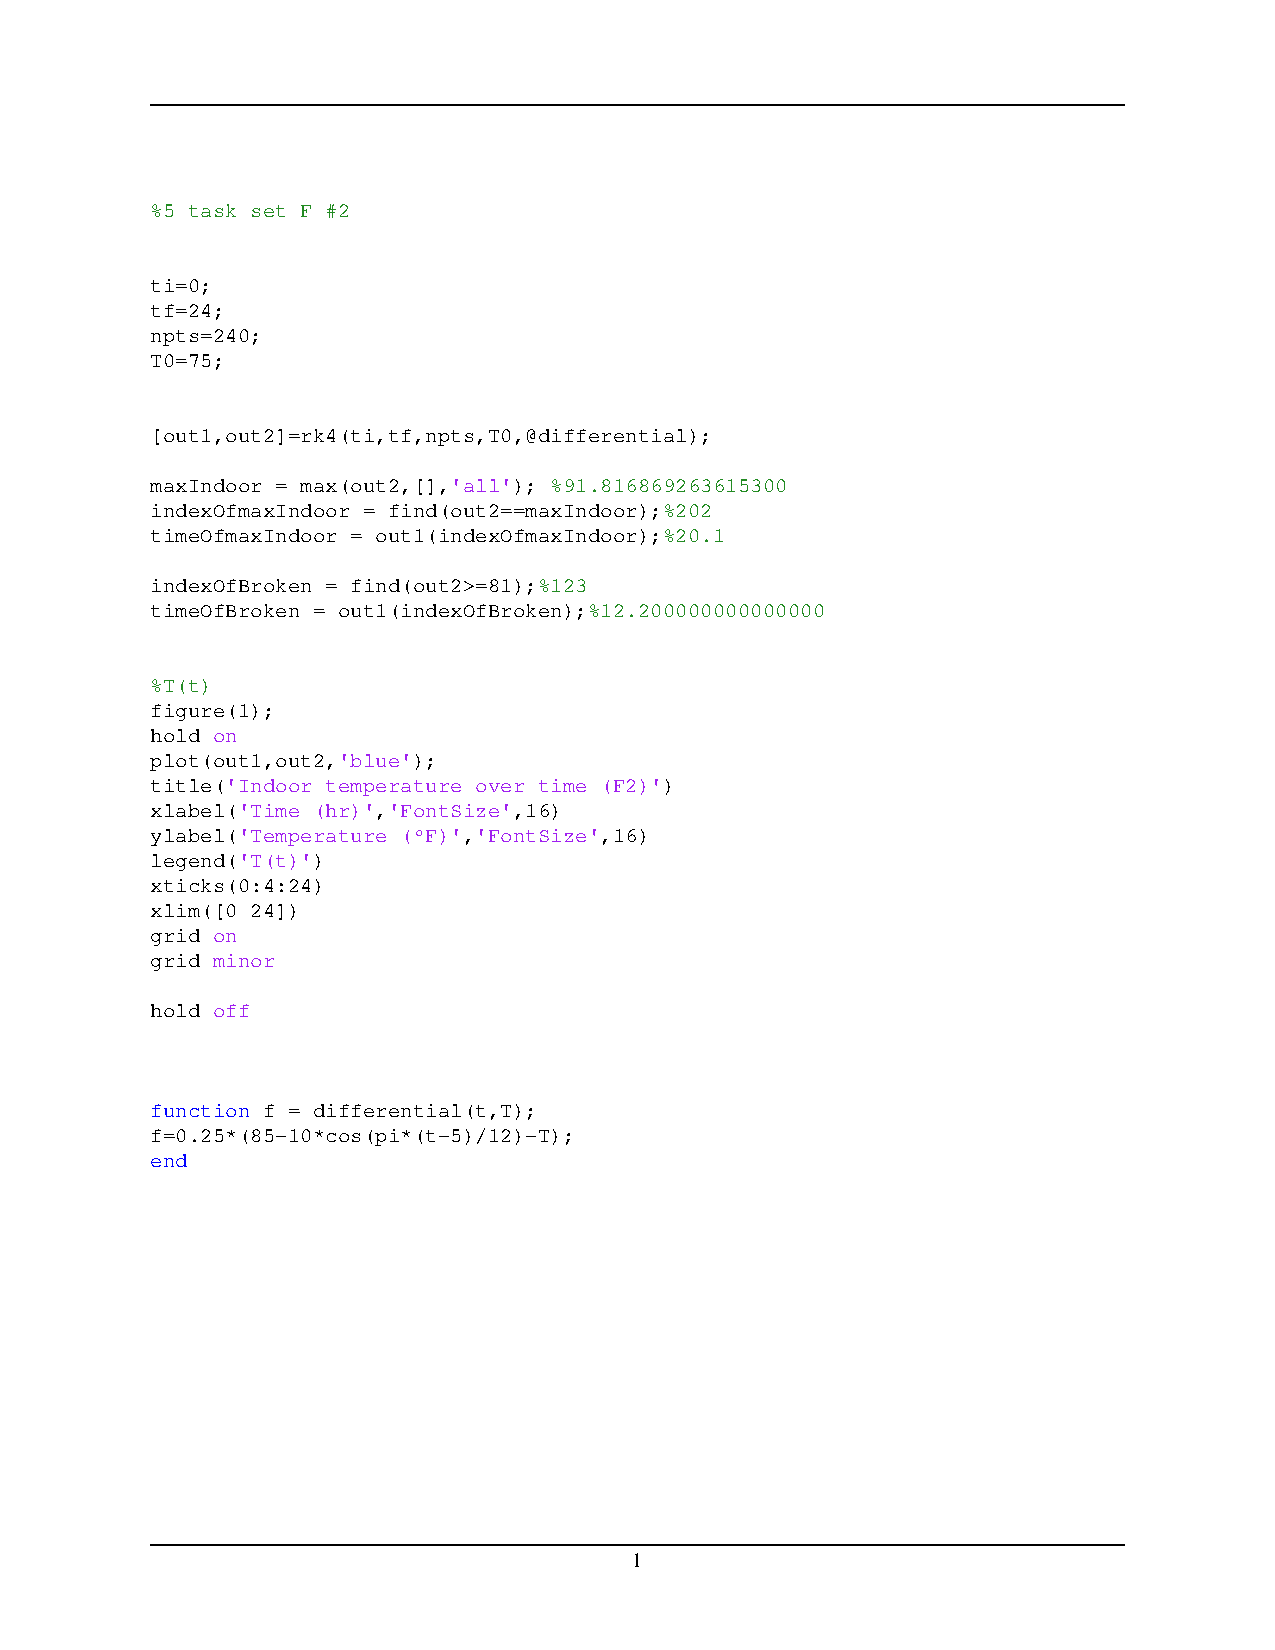
\includepdf[pages=-]{./codePdfs/DeProj1part5F2.pdf}
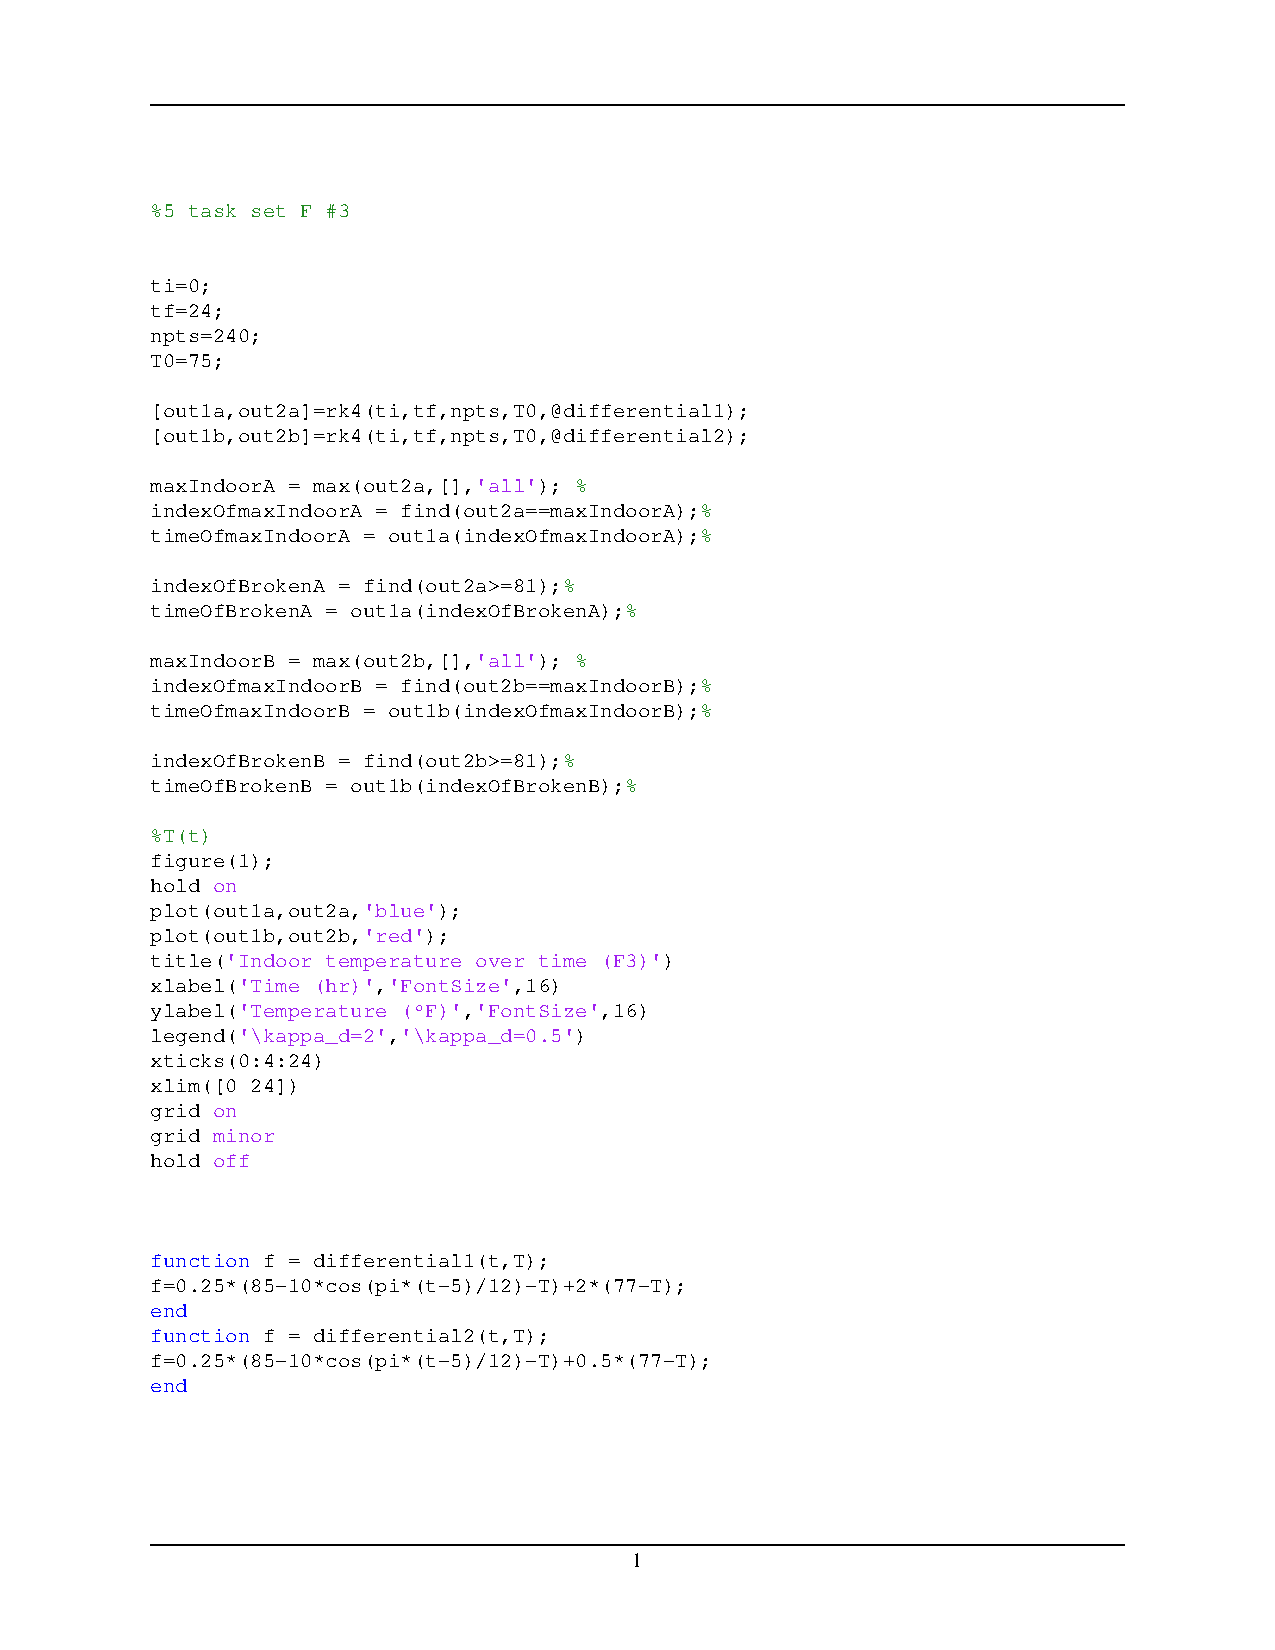
\includepdf[pages=-]{./codePdfs/DeProj1part5F3.pdf}
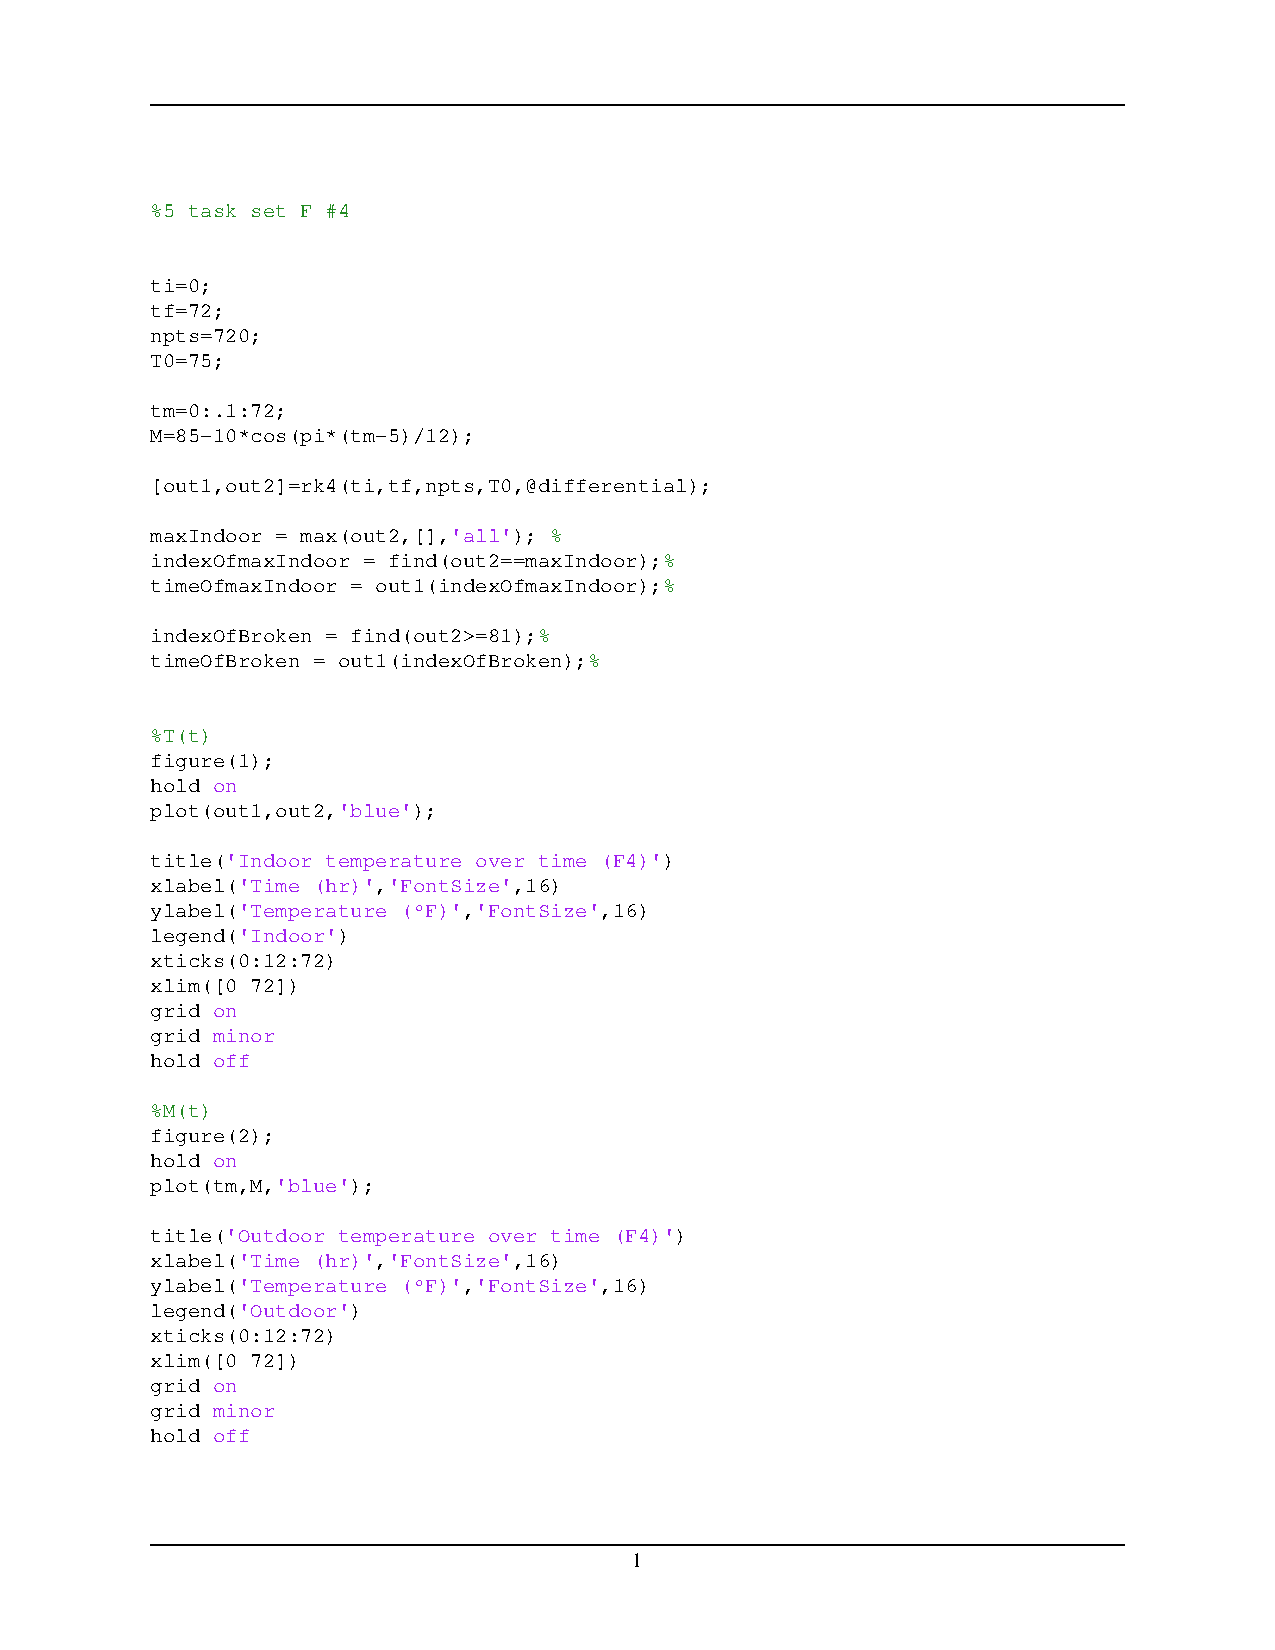
\includepdf[pages=-]{./codePdfs/DeProj1part5F4.pdf}



\end{document} % NOTHING AFTER THIS LINE IS PART OF THE DOCUMENT



